%%____________________________________________________________________________||
\section{Results}
\label{app:results}

\subsection{Tabulated presentation of results}
\label{app:results-tables}

\begin{table}[!h]
  \topcaption{
    Observed data counts and ``pre-fit'' background expectations in
    the signal region for the \texttt{eq1j} topology. The
    uncertainties in the background expectations include statistical
    as well as systematic contributions.
  }
  \label{tab:result-eq1j}
  \tiny
  \centering
  \begin{tabular}{rrllrrcl}
    \hline
    \njet\T\B & \nb & \scalht [GeV] & \mht [GeV] & Data & \multicolumn{3}{c}{SM} \\ 
    \hline
1 & 0 & $ 200- 400$ & $200-400$ & 291353 & 291377.9 &$\pm$&  975.0 \\
1 & 0 & $ 400- 600$ & $200-400$ &   8572 &   8542.8 &$\pm$&   88.0 \\
1 & 0 & $ 600- 900$ & $200-400$ &    878 &    878.5 &$\pm$&   30.6 \\
1 & 0 & $ 900- \infty$ & $200-400$ &     57 &     59.0 &$\pm$&    7.0 \\
1 & 1 & $ 200- 400$ & $200-400$ &  11072 &  11053.4 &$\pm$&  107.0 \\
1 & 1 & $ 400- 600$ & $200-400$ &    406 &    412.8 &$\pm$&   19.1 \\
1 & 1 & $ 600- \infty$ & $200-400$ &     71 &     72.2 &$\pm$&    8.4 \\
    \hline
  \end{tabular}
\end{table}

\begin{table}[!t]
  \topcaption{
    Observed data counts and ``pre-fit'' background expectations in
    the signal region for the \texttt{ge2a} topology. The
    uncertainties in the background expectations include statistical
    as well as systematic contributions.
  }
  \label{tab:result-ge2a}
  \tiny
  \centering
  \begin{tabular}{rrllrrcl}
    \hline
    \njet\T\B & \nb & \scalht [GeV] & \mht [GeV] & Data & \multicolumn{3}{c}{SM} \\ 
    \hline
$\geq 2${\it a} & 0 & $ 200- 400$ & $200-400$ & 116868 & 116789.5 &$\pm$&  547.3 \\
$\geq 2${\it a} & 0 & $ 200- 400$ & $400-600$ &      0 &      0.0 &$\pm$&    0.0 \\
$\geq 2${\it a} & 0 & $ 200- 400$ & $600-900$ &      0 &      0.0 &$\pm$&    0.0 \\
$\geq 2${\it a} & 0 & $ 200- 400$ & $900-\infty$ &      0 &      0.0 &$\pm$&    0.0 \\
$\geq 2${\it a} & 0 & $ 400- 600$ & $200-400$ &   2932 &   2932.3 &$\pm$&   47.7 \\
$\geq 2${\it a} & 0 & $ 400- 600$ & $400-600$ &   2800 &   2802.5 &$\pm$&   51.3 \\
$\geq 2${\it a} & 0 & $ 400- 600$ & $600-900$ &      0 &      0.0 &$\pm$&    0.0 \\
$\geq 2${\it a} & 0 & $ 400- 600$ & $900-\infty$ &      0 &      0.0 &$\pm$&    0.0 \\
$\geq 2${\it a} & 0 & $ 600- 900$ & $200-400$ &     67 &     65.1 &$\pm$&    5.9 \\
$\geq 2${\it a} & 0 & $ 600- 900$ & $400-600$ &     73 &     66.7 &$\pm$&    3.9 \\
$\geq 2${\it a} & 0 & $ 600- 900$ & $600-900$ &    177 &    188.0 &$\pm$&    9.7 \\
$\geq 2${\it a} & 0 & $ 600- 900$ & $900-\infty$ &      0 &      0.0 &$\pm$&    0.0 \\
$\geq 2${\it a} & 0 & $ 900- \infty$ & $200-400$ &     28 &     30.3 &$\pm$&    4.2 \\
$\geq 2${\it a} & 0 & $ 900- \infty$ & $400-600$ &     54 &     50.1 &$\pm$&    6.2 \\
$\geq 2${\it a} & 0 & $ 900- \infty$ & $600-900$ &      0 &      0.0 &$\pm$&    0.0 \\
$\geq 2${\it a} & 0 & $ 900- \infty$ & $900-\infty$ &      0 &      0.0 &$\pm$&    0.0 \\
$\geq 2${\it a} & 1 & $ 200- 400$ & $200-400$ &  16307 &  16370.7 &$\pm$&  129.2 \\
$\geq 2${\it a} & 1 & $ 200- 400$ & $400-600$ &      0 &      0.0 &$\pm$&    0.0 \\
$\geq 2${\it a} & 1 & $ 200- 400$ & $600-900$ &      0 &      0.0 &$\pm$&    0.0 \\
$\geq 2${\it a} & 1 & $ 200- 400$ & $900-\infty$ &      0 &      0.0 &$\pm$&    0.0 \\
$\geq 2${\it a} & 1 & $ 400- 600$ & $200-400$ &   1042 &   1079.9 &$\pm$&   24.0 \\
$\geq 2${\it a} & 1 & $ 400- 600$ & $400-600$ &    310 &    329.1 &$\pm$&   12.4 \\
$\geq 2${\it a} & 1 & $ 400- 600$ & $600-900$ &      0 &      0.0 &$\pm$&    0.0 \\
$\geq 2${\it a} & 1 & $ 400- 600$ & $900-\infty$ &      0 &      0.0 &$\pm$&    0.0 \\
$\geq 2${\it a} & 1 & $ 600- 900$ & $200-400$ &     12 &     20.6 &$\pm$&    2.1 \\
$\geq 2${\it a} & 1 & $ 600- 900$ & $400-600$ &     12 &     13.1 &$\pm$&    1.2 \\
$\geq 2${\it a} & 1 & $ 600- 900$ & $600-900$ &     22 &     23.0 &$\pm$&    2.7 \\
$\geq 2${\it a} & 1 & $ 600- 900$ & $900-\infty$ &      0 &      0.0 &$\pm$&    0.0 \\
$\geq 2${\it a} & 1 & $ 900- \infty$ & $200-400$ &      5 &      4.8 &$\pm$&    1.2 \\
$\geq 2${\it a} & 1 & $ 900- \infty$ & $400-600$ &      7 &      8.5 &$\pm$&    2.2 \\
$\geq 2${\it a} & 1 & $ 900- \infty$ & $600-900$ &      0 &      0.0 &$\pm$&    0.0 \\
$\geq 2${\it a} & 1 & $ 900- \infty$ & $900-\infty$ &      0 &      0.0 &$\pm$&    0.0 \\
$\geq 2${\it a} & 2 & $ 200- 400$ & $200-400$ &   2200 &   2173.8 &$\pm$&   31.5 \\
$\geq 2${\it a} & 2 & $ 200- 400$ & $400-600$ &      0 &      0.0 &$\pm$&    0.0 \\
$\geq 2${\it a} & 2 & $ 200- 400$ & $600-900$ &      0 &      0.0 &$\pm$&    0.0 \\
$\geq 2${\it a} & 2 & $ 200- 400$ & $900-\infty$ &      0 &      0.0 &$\pm$&    0.0 \\
$\geq 2${\it a} & 2 & $ 400- 600$ & $200-400$ &    410 &    392.6 &$\pm$&   11.4 \\
$\geq 2${\it a} & 2 & $ 400- 600$ & $400-600$ &     35 &     28.5 &$\pm$&    1.3 \\
$\geq 2${\it a} & 2 & $ 400- 600$ & $600-900$ &      0 &      0.0 &$\pm$&    0.0 \\
$\geq 2${\it a} & 2 & $ 400- 600$ & $900-\infty$ &      0 &      0.0 &$\pm$&    0.0 \\
$\geq 2${\it a} & 2 & $ 600- 900$ & $200-400$ &      5 &      6.3 &$\pm$&    0.8 \\
$\geq 2${\it a} & 2 & $ 600- 900$ & $400-600$ &      3 &      2.4 &$\pm$&    0.3 \\
$\geq 2${\it a} & 2 & $ 600- 900$ & $600-900$ &      2 &      1.8 &$\pm$&    0.2 \\
$\geq 2${\it a} & 2 & $ 600- 900$ & $900-\infty$ &      0 &      0.0 &$\pm$&    0.0 \\
$\geq 2${\it a} & 2 & $ 900- \infty$ & $200-400$ &      1 &      1.0 &$\pm$&    0.3 \\
$\geq 2${\it a} & 2 & $ 900- \infty$ & $400-600$ &      0 &      0.8 &$\pm$&    0.2 \\
$\geq 2${\it a} & 2 & $ 900- \infty$ & $600-900$ &      0 &      0.0 &$\pm$&    0.0 \\
$\geq 2${\it a} & 2 & $ 900- \infty$ & $900-\infty$ &      0 &      0.0 &$\pm$&    0.0 \\
$\geq 2${\it a} & 3 & $ 200- 400$ & $200-400$ &     92 &     80.1 &$\pm$&    5.4 \\
$\geq 2${\it a} & 3 & $ 200- 400$ & $400-600$ &      0 &      0.0 &$\pm$&    0.0 \\
$\geq 2${\it a} & 3 & $ 200- 400$ & $600-900$ &      0 &      0.0 &$\pm$&    0.0 \\
$\geq 2${\it a} & 3 & $ 200- 400$ & $900-\infty$ &      0 &      0.0 &$\pm$&    0.0 \\
$\geq 2${\it a} & 3 & $ 400- 600$ & $200-400$ &     38 &     40.2 &$\pm$&    3.1 \\
$\geq 2${\it a} & 3 & $ 400- 600$ & $400-600$ &      2 &      0.9 &$\pm$&    0.1 \\
$\geq 2${\it a} & 3 & $ 400- 600$ & $600-900$ &      0 &      0.0 &$\pm$&    0.0 \\
$\geq 2${\it a} & 3 & $ 400- 600$ & $900-\infty$ &      0 &      0.0 &$\pm$&    0.0 \\
$\geq 2${\it a} & 3 & $ 600- \infty$ & $200-400$ &      1 &      1.4 &$\pm$&    0.3 \\
$\geq 2${\it a} & 3 & $ 600- \infty$ & $400-600$ &      0 &      0.3 &$\pm$&    0.1 \\
$\geq 2${\it a} & 3 & $ 600- \infty$ & $600-900$ &      0 &      0.2 &$\pm$&    0.0 \\
$\geq 2${\it a} & 3 & $ 600- \infty$ & $900-\infty$ &      0 &      0.0 &$\pm$&    0.0 \\
    \hline
  \end{tabular}
\end{table}

\begin{table}[!t]
  \topcaption{
    Observed data counts and ``pre-fit'' background expectations in
    the signal region for the \texttt{eq2j} topology. The
    uncertainties in the background expectations include statistical
    as well as systematic contributions. 
  }
  \label{tab:result-eq2j}
  \tiny
  \centering
  \begin{tabular}{rrllrrcl}
    \hline
    \njet\T\B & \nb & \scalht [GeV] & \mht [GeV] & Data & \multicolumn{3}{c}{SM} \\ 
    \hline
2 & 0 & $ 200- 400$ & $200-400$ &  34934 &  34885.3 &$\pm$&  208.9 \\
2 & 0 & $ 200- 400$ & $400-600$ &      0 &      0.0 &$\pm$&    0.0 \\
2 & 0 & $ 200- 400$ & $600-900$ &      0 &      0.0 &$\pm$&    0.0 \\
2 & 0 & $ 200- 400$ & $900-\infty$ &      0 &      0.0 &$\pm$&    0.0 \\
2 & 0 & $ 400- 600$ & $200-400$ &   3468 &   3451.3 &$\pm$&  122.2 \\
2 & 0 & $ 400- 600$ & $400-600$ &   2568 &   2522.5 &$\pm$&   82.5 \\
2 & 0 & $ 400- 600$ & $600-900$ &      0 &      0.0 &$\pm$&    0.0 \\
2 & 0 & $ 400- 600$ & $900-\infty$ &      0 &      0.0 &$\pm$&    0.0 \\
2 & 0 & $ 600- 900$ & $200-400$ &    226 &    237.8 &$\pm$&   11.1 \\
2 & 0 & $ 600- 900$ & $400-600$ &    253 &    271.1 &$\pm$&    8.6 \\
2 & 0 & $ 600- 900$ & $600-900$ &    303 &    319.3 &$\pm$&   12.8 \\
2 & 0 & $ 600- 900$ & $900-\infty$ &      0 &      0.0 &$\pm$&    0.0 \\
2 & 0 & $ 900-1200$ & $200-400$ &    165 &    164.7 &$\pm$&    9.8 \\
2 & 0 & $ 900-1200$ & $400-600$ &    125 &    127.4 &$\pm$&    6.2 \\
2 & 0 & $ 900-1200$ & $600-900$ &     97 &     84.3 &$\pm$&    4.8 \\
2 & 0 & $ 900-1200$ & $900-\infty$ &     25 &     33.2 &$\pm$&    2.9 \\
2 & 0 & $1200- \infty$ & $200-400$ &      9 &      7.4 &$\pm$&    1.0 \\
2 & 0 & $1200- \infty$ & $400-600$ &     26 &     23.4 &$\pm$&    2.5 \\
2 & 0 & $1200- \infty$ & $600-900$ &     22 &     22.2 &$\pm$&    2.2 \\
2 & 0 & $1200- \infty$ & $900-\infty$ &     19 &     19.1 &$\pm$&    2.4 \\
2 & 1 & $ 200- 400$ & $200-400$ &   3850 &   3895.9 &$\pm$&   59.6 \\
2 & 1 & $ 200- 400$ & $400-600$ &      0 &      0.0 &$\pm$&    0.0 \\
2 & 1 & $ 200- 400$ & $600-900$ &      0 &      0.0 &$\pm$&    0.0 \\
2 & 1 & $ 200- 400$ & $900-\infty$ &      0 &      0.0 &$\pm$&    0.0 \\
2 & 1 & $ 400- 600$ & $200-400$ &    327 &    324.1 &$\pm$&   16.4 \\
2 & 1 & $ 400- 600$ & $400-600$ &    240 &    268.6 &$\pm$&   10.9 \\
2 & 1 & $ 400- 600$ & $600-900$ &      0 &      0.0 &$\pm$&    0.0 \\
2 & 1 & $ 400- 600$ & $900-\infty$ &      0 &      0.0 &$\pm$&    0.0 \\
2 & 1 & $ 600- 900$ & $200-400$ &     22 &     28.0 &$\pm$&    2.3 \\
2 & 1 & $ 600- 900$ & $400-600$ &     39 &     31.1 &$\pm$&    2.6 \\
2 & 1 & $ 600- 900$ & $600-900$ &     31 &     36.5 &$\pm$&    3.0 \\
2 & 1 & $ 600- 900$ & $900-\infty$ &      0 &      0.0 &$\pm$&    0.0 \\
2 & 1 & $ 900-1200$ & $200-400$ &     17 &     21.1 &$\pm$&    2.5 \\
2 & 1 & $ 900-1200$ & $400-600$ &     15 &     17.6 &$\pm$&    2.1 \\
2 & 1 & $ 900-1200$ & $600-900$ &     12 &     10.2 &$\pm$&    1.5 \\
2 & 1 & $ 900-1200$ & $900-\infty$ &      6 &      4.7 &$\pm$&    0.8 \\
2 & 1 & $1200- \infty$ & $200-400$ &      1 &      1.1 &$\pm$&    0.3 \\
2 & 1 & $1200- \infty$ & $400-600$ &      6 &      3.6 &$\pm$&    0.9 \\
2 & 1 & $1200- \infty$ & $600-900$ &      1 &      2.5 &$\pm$&    0.7 \\
2 & 1 & $1200- \infty$ & $900-\infty$ &      4 &      2.7 &$\pm$&    0.8 \\
2 & 2 & $ 200- 400$ & $200-400$ &    254 &    250.6 &$\pm$&    9.2 \\
2 & 2 & $ 200- 400$ & $400-600$ &      0 &      0.0 &$\pm$&    0.0 \\
2 & 2 & $ 200- 400$ & $600-900$ &      0 &      0.0 &$\pm$&    0.0 \\
2 & 2 & $ 200- 400$ & $900-\infty$ &      0 &      0.0 &$\pm$&    0.0 \\
2 & 2 & $ 400- 600$ & $200-400$ &     22 &     15.1 &$\pm$&    1.1 \\
2 & 2 & $ 400- 600$ & $400-600$ &     18 &     18.5 &$\pm$&    1.2 \\
2 & 2 & $ 400- 600$ & $600-900$ &      0 &      0.0 &$\pm$&    0.0 \\
2 & 2 & $ 400- 600$ & $900-\infty$ &      0 &      0.0 &$\pm$&    0.0 \\
2 & 2 & $ 600- \infty$ & $200-400$ &      1 &      1.7 &$\pm$&    0.2 \\
2 & 2 & $ 600- \infty$ & $400-600$ &      2 &      2.1 &$\pm$&    0.2 \\
2 & 2 & $ 600- \infty$ & $600-900$ &      2 &      3.0 &$\pm$&    0.3 \\
2 & 2 & $ 600- \infty$ & $900-\infty$ &      0 &      0.0 &$\pm$&    0.0 \\
    \hline
  \end{tabular}
\end{table}

\begin{table}[!t]
  \topcaption{
    Observed data counts and ``pre-fit'' background expectations in
    the signal region for the \texttt{eq3j} topology. The
    uncertainties in the background expectations include statistical
    as well as systematic contributions. 
  }
  \label{tab:result-eq3j}
  \tiny
  \centering
  \begin{tabular}{rrllrrcl}
    \hline
    \njet\T\B & \nb & \scalht [GeV] & \mht [GeV] & Data & \multicolumn{3}{c}{SM} \\ 
    \hline
3 & 0 & $ 200- 400$ & $200-400$ &  11815 &  11888.1 &$\pm$&  117.9 \\
3 & 0 & $ 200- 400$ & $400-600$ &      0 &      0.0 &$\pm$&    0.0 \\
3 & 0 & $ 200- 400$ & $600-900$ &      0 &      0.0 &$\pm$&    0.0 \\
3 & 0 & $ 200- 400$ & $900-\infty$ &      0 &      0.0 &$\pm$&    0.0 \\
3 & 0 & $ 400- 600$ & $200-400$ &   7120 &   7102.9 &$\pm$&   89.7 \\
3 & 0 & $ 400- 600$ & $400-600$ &   1463 &   1474.7 &$\pm$&   34.4 \\
3 & 0 & $ 400- 600$ & $600-900$ &      0 &      0.0 &$\pm$&    0.0 \\
3 & 0 & $ 400- 600$ & $900-\infty$ &      0 &      0.0 &$\pm$&    0.0 \\
3 & 0 & $ 600- 900$ & $200-400$ &    668 &    648.5 &$\pm$&   19.2 \\
3 & 0 & $ 600- 900$ & $400-600$ &    593 &    575.6 &$\pm$&   17.3 \\
3 & 0 & $ 600- 900$ & $600-900$ &    246 &    240.9 &$\pm$&   10.4 \\
3 & 0 & $ 600- 900$ & $900-\infty$ &      0 &      0.0 &$\pm$&    0.0 \\
3 & 0 & $ 900-1200$ & $200-400$ &    245 &    242.9 &$\pm$&   11.8 \\
3 & 0 & $ 900-1200$ & $400-600$ &    164 &    158.6 &$\pm$&    7.8 \\
3 & 0 & $ 900-1200$ & $600-900$ &    101 &     99.9 &$\pm$&    5.8 \\
3 & 0 & $ 900-1200$ & $900-\infty$ &     19 &     24.4 &$\pm$&    2.3 \\
3 & 0 & $1200- \infty$ & $200-400$ &     21 &     15.7 &$\pm$&    1.7 \\
3 & 0 & $1200- \infty$ & $400-600$ &     28 &     38.6 &$\pm$&    2.9 \\
3 & 0 & $1200- \infty$ & $600-900$ &     31 &     27.9 &$\pm$&    2.2 \\
3 & 0 & $1200- \infty$ & $900-\infty$ &     17 &     18.6 &$\pm$&    2.0 \\
3 & 1 & $ 200- 400$ & $200-400$ &   2703 &   2692.7 &$\pm$&   44.2 \\
3 & 1 & $ 200- 400$ & $400-600$ &      0 &      0.0 &$\pm$&    0.0 \\
3 & 1 & $ 200- 400$ & $600-900$ &      0 &      0.0 &$\pm$&    0.0 \\
3 & 1 & $ 200- 400$ & $900-\infty$ &      0 &      0.0 &$\pm$&    0.0 \\
3 & 1 & $ 400- 600$ & $200-400$ &   1212 &   1269.6 &$\pm$&   29.1 \\
3 & 1 & $ 400- 600$ & $400-600$ &    301 &    268.6 &$\pm$&    9.8 \\
3 & 1 & $ 400- 600$ & $600-900$ &      0 &      0.0 &$\pm$&    0.0 \\
3 & 1 & $ 400- 600$ & $900-\infty$ &      0 &      0.0 &$\pm$&    0.0 \\
3 & 1 & $ 600- 900$ & $200-400$ &    110 &    104.3 &$\pm$&    5.5 \\
3 & 1 & $ 600- 900$ & $400-600$ &     96 &     90.4 &$\pm$&    5.1 \\
3 & 1 & $ 600- 900$ & $600-900$ &     42 &     39.3 &$\pm$&    2.6 \\
3 & 1 & $ 600- 900$ & $900-\infty$ &      0 &      0.0 &$\pm$&    0.0 \\
3 & 1 & $ 900-1200$ & $200-400$ &     39 &     41.3 &$\pm$&    4.0 \\
3 & 1 & $ 900-1200$ & $400-600$ &     24 &     24.3 &$\pm$&    2.2 \\
3 & 1 & $ 900-1200$ & $600-900$ &     10 &     16.0 &$\pm$&    1.8 \\
3 & 1 & $ 900-1200$ & $900-\infty$ &      6 &      5.3 &$\pm$&    1.2 \\
3 & 1 & $1200- \infty$ & $200-400$ &      3 &      2.8 &$\pm$&    0.5 \\
3 & 1 & $1200- \infty$ & $400-600$ &      5 &      6.4 &$\pm$&    1.1 \\
3 & 1 & $1200- \infty$ & $600-900$ &      7 &      4.7 &$\pm$&    0.9 \\
3 & 1 & $1200- \infty$ & $900-\infty$ &      4 &      3.4 &$\pm$&    0.8 \\
3 & 2 & $ 200- 400$ & $200-400$ &    495 &    480.1 &$\pm$&   14.3 \\
3 & 2 & $ 200- 400$ & $400-600$ &      0 &      0.0 &$\pm$&    0.0 \\
3 & 2 & $ 200- 400$ & $600-900$ &      0 &      0.0 &$\pm$&    0.0 \\
3 & 2 & $ 200- 400$ & $900-\infty$ &      0 &      0.0 &$\pm$&    0.0 \\
3 & 2 & $ 400- 600$ & $200-400$ &    229 &    220.5 &$\pm$&    6.6 \\
3 & 2 & $ 400- 600$ & $400-600$ &     34 &     31.8 &$\pm$&    1.2 \\
3 & 2 & $ 400- 600$ & $600-900$ &      0 &      0.0 &$\pm$&    0.0 \\
3 & 2 & $ 400- 600$ & $900-\infty$ &      0 &      0.0 &$\pm$&    0.0 \\
3 & 2 & $ 600- 900$ & $200-400$ &     10 &      9.7 &$\pm$&    0.6 \\
3 & 2 & $ 600- 900$ & $400-600$ &      9 &     10.3 &$\pm$&    0.6 \\
3 & 2 & $ 600- 900$ & $600-900$ &      2 &      3.8 &$\pm$&    0.3 \\
3 & 2 & $ 600- 900$ & $900-\infty$ &      0 &      0.0 &$\pm$&    0.0 \\
3 & 2 & $ 900-1200$ & $200-400$ &      4 &      3.7 &$\pm$&    0.4 \\
3 & 2 & $ 900-1200$ & $400-600$ &      2 &      1.9 &$\pm$&    0.2 \\
3 & 2 & $ 900-1200$ & $600-900$ &      2 &      1.4 &$\pm$&    0.2 \\
3 & 2 & $ 900-1200$ & $900-\infty$ &      0 &      0.5 &$\pm$&    0.1 \\
3 & 2 & $1200- \infty$ & $200-400$ &      1 &      0.3 &$\pm$&    0.1 \\
3 & 2 & $1200- \infty$ & $400-600$ &      0 &      0.7 &$\pm$&    0.1 \\
3 & 2 & $1200- \infty$ & $600-900$ &      0 &      0.5 &$\pm$&    0.1 \\
3 & 2 & $1200- \infty$ & $900-\infty$ &      0 &      0.3 &$\pm$&    0.1 \\
3 & 3 & $ 200- 400$ & $200-400$ &     16 &     14.9 &$\pm$&    2.2 \\
3 & 3 & $ 200- 400$ & $400-600$ &      0 &      0.0 &$\pm$&    0.0 \\
3 & 3 & $ 200- 400$ & $600-900$ &      0 &      0.0 &$\pm$&    0.0 \\
3 & 3 & $ 200- 400$ & $900-\infty$ &      0 &      0.0 &$\pm$&    0.0 \\
3 & 3 & $ 400- 600$ & $200-400$ &     10 &      6.7 &$\pm$&    1.1 \\
3 & 3 & $ 400- 600$ & $400-600$ &      2 &      0.8 &$\pm$&    0.1 \\
3 & 3 & $ 400- 600$ & $600-900$ &      0 &      0.0 &$\pm$&    0.0 \\
3 & 3 & $ 400- 600$ & $900-\infty$ &      0 &      0.0 &$\pm$&    0.0 \\
3 & 3 & $ 600- \infty$ & $200-400$ &      3 &      0.4 &$\pm$&    0.0 \\
3 & 3 & $ 600- \infty$ & $400-600$ &      3 &      0.4 &$\pm$&    0.1 \\
3 & 3 & $ 600- \infty$ & $600-900$ &      0 &      0.2 &$\pm$&    0.0 \\
3 & 3 & $ 600- \infty$ & $900-\infty$ &      0 &      0.0 &$\pm$&    0.0 \\
    \hline
  \end{tabular}
\end{table}

\begin{table}[!t]
  \topcaption{
    Observed data counts and ``pre-fit'' background expectations in
    the signal region for the \texttt{eq4j} topology. The
    uncertainties in the background expectations include statistical
    as well as systematic contributions. 
  }
  \label{tab:result-eq4j}
  \tiny
  \centering
  \begin{tabular}{rrllrrcl}
    \hline
    \njet\T\B & \nb & \scalht [GeV] & \mht [GeV] & Data & \multicolumn{3}{c}{SM} \\ 
    \hline
4 & 0 & $ 400- 600$ & $200-400$ &   4324 &   4329.3 &$\pm$&   61.8 \\
4 & 0 & $ 400- 600$ & $400-600$ &    437 &    436.9 &$\pm$&   17.3 \\
4 & 0 & $ 400- 600$ & $600-900$ &      0 &      0.0 &$\pm$&    0.0 \\
4 & 0 & $ 400- 600$ & $900-\infty$ &      0 &      0.0 &$\pm$&    0.0 \\
4 & 0 & $ 600- 900$ & $200-400$ &    751 &    746.9 &$\pm$&   20.6 \\
4 & 0 & $ 600- 900$ & $400-600$ &    484 &    472.8 &$\pm$&   17.1 \\
4 & 0 & $ 600- 900$ & $600-900$ &    110 &    100.3 &$\pm$&    6.4 \\
4 & 0 & $ 600- 900$ & $900-\infty$ &      0 &      0.0 &$\pm$&    0.0 \\
4 & 0 & $ 900-1200$ & $200-400$ &    186 &    183.5 &$\pm$&    9.0 \\
4 & 0 & $ 900-1200$ & $400-600$ &    111 &    109.8 &$\pm$&    5.8 \\
4 & 0 & $ 900-1200$ & $600-900$ &     66 &     60.3 &$\pm$&    4.2 \\
4 & 0 & $ 900-1200$ & $900-\infty$ &     13 &      8.8 &$\pm$&    1.1 \\
4 & 0 & $1200- \infty$ & $200-400$ &     13 &     16.5 &$\pm$&    1.9 \\
4 & 0 & $1200- \infty$ & $400-600$ &     32 &     35.0 &$\pm$&    2.8 \\
4 & 0 & $1200- \infty$ & $600-900$ &     28 &     25.4 &$\pm$&    2.2 \\
4 & 0 & $1200- \infty$ & $900-\infty$ &     15 &     15.9 &$\pm$&    1.7 \\
4 & 1 & $ 400- 600$ & $200-400$ &   1497 &   1504.2 &$\pm$&   29.4 \\
4 & 1 & $ 400- 600$ & $400-600$ &    109 &    121.9 &$\pm$&    5.8 \\
4 & 1 & $ 400- 600$ & $600-900$ &      0 &      0.0 &$\pm$&    0.0 \\
4 & 1 & $ 400- 600$ & $900-\infty$ &      0 &      0.0 &$\pm$&    0.0 \\
4 & 1 & $ 600- 900$ & $200-400$ &    184 &    198.7 &$\pm$&    8.0 \\
4 & 1 & $ 600- 900$ & $400-600$ &    106 &    114.2 &$\pm$&    5.5 \\
4 & 1 & $ 600- 900$ & $600-900$ &     19 &     20.6 &$\pm$&    1.6 \\
4 & 1 & $ 600- 900$ & $900-\infty$ &      0 &      0.0 &$\pm$&    0.0 \\
4 & 1 & $ 900-1200$ & $200-400$ &     60 &     46.3 &$\pm$&    3.7 \\
4 & 1 & $ 900-1200$ & $400-600$ &     19 &     24.5 &$\pm$&    2.3 \\
4 & 1 & $ 900-1200$ & $600-900$ &     11 &     11.3 &$\pm$&    1.4 \\
4 & 1 & $ 900-1200$ & $900-\infty$ &      1 &      1.4 &$\pm$&    0.3 \\
4 & 1 & $1200- \infty$ & $200-400$ &      7 &      5.3 &$\pm$&    0.8 \\
4 & 1 & $1200- \infty$ & $400-600$ &     11 &     12.4 &$\pm$&    1.5 \\
4 & 1 & $1200- \infty$ & $600-900$ &      7 &      6.4 &$\pm$&    0.9 \\
4 & 1 & $1200- \infty$ & $900-\infty$ &      4 &      4.5 &$\pm$&    0.8 \\
4 & 2 & $ 400- 600$ & $200-400$ &    524 &    506.3 &$\pm$&   14.9 \\
4 & 2 & $ 400- 600$ & $400-600$ &     29 &     26.6 &$\pm$&    1.4 \\
4 & 2 & $ 400- 600$ & $600-900$ &      0 &      0.0 &$\pm$&    0.0 \\
4 & 2 & $ 400- 600$ & $900-\infty$ &      0 &      0.0 &$\pm$&    0.0 \\
4 & 2 & $ 600- 900$ & $200-400$ &     50 &     38.3 &$\pm$&    1.8 \\
4 & 2 & $ 600- 900$ & $400-600$ &     19 &     21.1 &$\pm$&    1.1 \\
4 & 2 & $ 600- 900$ & $600-900$ &      1 &      2.9 &$\pm$&    0.2 \\
4 & 2 & $ 600- 900$ & $900-\infty$ &      0 &      0.0 &$\pm$&    0.0 \\
4 & 2 & $ 900-1200$ & $200-400$ &     10 &      7.6 &$\pm$&    0.7 \\
4 & 2 & $ 900-1200$ & $400-600$ &      7 &      3.8 &$\pm$&    0.4 \\
4 & 2 & $ 900-1200$ & $600-900$ &      0 &      1.5 &$\pm$&    0.2 \\
4 & 2 & $ 900-1200$ & $900-\infty$ &      1 &      0.2 &$\pm$&    0.1 \\
4 & 2 & $1200- \infty$ & $200-400$ &      1 &      0.7 &$\pm$&    0.1 \\
4 & 2 & $1200- \infty$ & $400-600$ &      0 &      1.7 &$\pm$&    0.2 \\
4 & 2 & $1200- \infty$ & $600-900$ &      0 &      0.7 &$\pm$&    0.1 \\
4 & 2 & $1200- \infty$ & $900-\infty$ &      1 &      0.6 &$\pm$&    0.1 \\
4 & 3 & $ 400- 600$ & $200-400$ &     35 &     42.1 &$\pm$&    3.2 \\
4 & 3 & $ 400- 600$ & $400-600$ &      1 &      2.0 &$\pm$&    0.2 \\
4 & 3 & $ 400- 600$ & $600-900$ &      0 &      0.0 &$\pm$&    0.0 \\
4 & 3 & $ 400- 600$ & $900-\infty$ &      0 &      0.0 &$\pm$&    0.0 \\
4 & 3 & $ 600- 900$ & $200-400$ &      6 &      3.3 &$\pm$&    0.4 \\
4 & 3 & $ 600- 900$ & $400-600$ &      0 &      1.6 &$\pm$&    0.2 \\
4 & 3 & $ 600- 900$ & $600-900$ &      0 &      0.2 &$\pm$&    0.0 \\
4 & 3 & $ 600- 900$ & $900-\infty$ &      0 &      0.0 &$\pm$&    0.0 \\
4 & 3 & $ 900- \infty$ & $200-400$ &      0 &      0.7 &$\pm$&    0.2 \\
4 & 3 & $ 900- \infty$ & $400-600$ &      0 &      0.4 &$\pm$&    0.1 \\
4 & 3 & $ 900- \infty$ & $600-900$ &      0 &      0.2 &$\pm$&    0.0 \\
4 & 3 & $ 900- \infty$ & $900-\infty$ &      0 &      0.0 &$\pm$&    0.0 \\
    \hline
  \end{tabular}
\end{table}

\begin{table}[!t]
  \topcaption{
    Observed data counts and ``pre-fit'' background expectations in
    the signal region for the \texttt{eq5j} topology. The
    uncertainties in the background expectations include statistical
    as well as systematic contributions. 
  }
  \label{tab:result-eq5j}
  \tiny
  \centering
  \begin{tabular}{rrllrrcl}
    \hline
    \njet\T\B & \nb & \scalht [GeV] & \mht [GeV] & Data & \multicolumn{3}{c}{SM} \\ 
    \hline
5 & 0 & $ 400- 600$ & $200-400$ &   1132 &   1112.7 &$\pm$&   28.3 \\
5 & 0 & $ 400- 600$ & $400-600$ &     59 &     71.2 &$\pm$&    5.8 \\
5 & 0 & $ 400- 600$ & $600-900$ &      0 &      0.0 &$\pm$&    0.0 \\
5 & 0 & $ 400- 600$ & $900-\infty$ &      0 &      0.0 &$\pm$&    0.0 \\
5 & 0 & $ 600- 900$ & $200-400$ &    435 &    471.0 &$\pm$&   16.9 \\
5 & 0 & $ 600- 900$ & $400-600$ &    201 &    186.9 &$\pm$&    9.6 \\
5 & 0 & $ 600- 900$ & $600-900$ &     17 &     26.7 &$\pm$&    2.5 \\
5 & 0 & $ 600- 900$ & $900-\infty$ &      0 &      0.0 &$\pm$&    0.0 \\
5 & 0 & $ 900-1200$ & $200-400$ &    124 &    120.9 &$\pm$&    8.6 \\
5 & 0 & $ 900-1200$ & $400-600$ &     59 &     57.8 &$\pm$&    4.7 \\
5 & 0 & $ 900-1200$ & $600-900$ &     28 &     28.6 &$\pm$&    3.8 \\
5 & 0 & $ 900-1200$ & $900-\infty$ &      0 &      0.0 &$\pm$&    0.0 \\
5 & 0 & $1200- \infty$ & $200-400$ &      7 &      9.8 &$\pm$&    1.4 \\
5 & 0 & $1200- \infty$ & $400-600$ &     16 &     14.2 &$\pm$&    1.8 \\
5 & 0 & $1200- \infty$ & $600-900$ &      7 &      9.2 &$\pm$&    1.4 \\
5 & 0 & $1200- \infty$ & $900-\infty$ &      6 &      4.9 &$\pm$&    0.9 \\
5 & 1 & $ 400- 600$ & $200-400$ &    591 &    585.8 &$\pm$&   20.4 \\
5 & 1 & $ 400- 600$ & $400-600$ &     22 &     23.6 &$\pm$&    2.1 \\
5 & 1 & $ 400- 600$ & $600-900$ &      0 &      0.0 &$\pm$&    0.0 \\
5 & 1 & $ 400- 600$ & $900-\infty$ &      0 &      0.0 &$\pm$&    0.0 \\
5 & 1 & $ 600- 900$ & $200-400$ &    198 &    178.5 &$\pm$&    7.4 \\
5 & 1 & $ 600- 900$ & $400-600$ &     50 &     55.8 &$\pm$&    3.4 \\
5 & 1 & $ 600- 900$ & $600-900$ &     11 &      6.9 &$\pm$&    0.8 \\
5 & 1 & $ 600- 900$ & $900-\infty$ &      0 &      0.0 &$\pm$&    0.0 \\
5 & 1 & $ 900-1200$ & $200-400$ &     33 &     39.3 &$\pm$&    3.4 \\
5 & 1 & $ 900-1200$ & $400-600$ &     15 &     18.3 &$\pm$&    2.0 \\
5 & 1 & $ 900-1200$ & $600-900$ &      9 &      8.3 &$\pm$&    1.2 \\
5 & 1 & $ 900-1200$ & $900-\infty$ &      0 &      0.0 &$\pm$&    0.0 \\
5 & 1 & $1200- \infty$ & $200-400$ &      4 &      3.4 &$\pm$&    0.6 \\
5 & 1 & $1200- \infty$ & $400-600$ &      3 &      5.3 &$\pm$&    1.0 \\
5 & 1 & $1200- \infty$ & $600-900$ &      5 &      2.9 &$\pm$&    0.6 \\
5 & 1 & $1200- \infty$ & $900-\infty$ &      2 &      1.9 &$\pm$&    0.5 \\
5 & 2 & $ 400- 600$ & $200-400$ &    284 &    275.8 &$\pm$&   10.7 \\
5 & 2 & $ 400- 600$ & $400-600$ &     10 &      5.3 &$\pm$&    0.4 \\
5 & 2 & $ 400- 600$ & $600-900$ &      0 &      0.0 &$\pm$&    0.0 \\
5 & 2 & $ 400- 600$ & $900-\infty$ &      0 &      0.0 &$\pm$&    0.0 \\
5 & 2 & $ 600- 900$ & $200-400$ &     63 &     68.3 &$\pm$&    3.6 \\
5 & 2 & $ 600- 900$ & $400-600$ &     16 &     17.6 &$\pm$&    1.1 \\
5 & 2 & $ 600- 900$ & $600-900$ &      0 &      1.6 &$\pm$&    0.2 \\
5 & 2 & $ 600- 900$ & $900-\infty$ &      0 &      0.0 &$\pm$&    0.0 \\
5 & 2 & $ 900-1200$ & $200-400$ &      5 &      9.8 &$\pm$&    1.0 \\
5 & 2 & $ 900-1200$ & $400-600$ &      5 &      3.6 &$\pm$&    0.4 \\
5 & 2 & $ 900-1200$ & $600-900$ &      1 &      1.8 &$\pm$&    0.3 \\
5 & 2 & $ 900-1200$ & $900-\infty$ &      0 &      0.0 &$\pm$&    0.0 \\
5 & 2 & $1200- \infty$ & $200-400$ &      0 &      0.7 &$\pm$&    0.1 \\
5 & 2 & $1200- \infty$ & $400-600$ &      2 &      1.0 &$\pm$&    0.2 \\
5 & 2 & $1200- \infty$ & $600-900$ &      1 &      0.4 &$\pm$&    0.1 \\
5 & 2 & $1200- \infty$ & $900-\infty$ &      1 &      0.3 &$\pm$&    0.1 \\
5 & 3 & $ 400- 600$ & $200-400$ &     25 &     31.3 &$\pm$&    3.0 \\
5 & 3 & $ 400- 600$ & $400-600$ &      1 &      0.4 &$\pm$&    0.0 \\
5 & 3 & $ 400- 600$ & $600-900$ &      0 &      0.0 &$\pm$&    0.0 \\
5 & 3 & $ 400- 600$ & $900-\infty$ &      0 &      0.0 &$\pm$&    0.0 \\
5 & 3 & $ 600- 900$ & $200-400$ &      7 &      7.6 &$\pm$&    0.9 \\
5 & 3 & $ 600- 900$ & $400-600$ &      3 &      1.7 &$\pm$&    0.2 \\
5 & 3 & $ 600- 900$ & $600-900$ &      0 &      0.1 &$\pm$&    0.0 \\
5 & 3 & $ 600- 900$ & $900-\infty$ &      0 &      0.0 &$\pm$&    0.0 \\
5 & 3 & $ 900- \infty$ & $200-400$ &      0 &      0.8 &$\pm$&    0.2 \\
5 & 3 & $ 900- \infty$ & $400-600$ &      0 &      0.4 &$\pm$&    0.1 \\
5 & 3 & $ 900- \infty$ & $600-900$ &      0 &      0.2 &$\pm$&    0.0 \\
5 & 3 & $ 900- \infty$ & $900-\infty$ &      0 &      0.0 &$\pm$&    0.0 \\
5 & $\geq 4$ & $ 400- \infty$ & $200-400$ &      2 &      1.8 &$\pm$&    0.5 \\
5 & $\geq 4$ & $ 400- \infty$ & $400-600$ &      1 &      0.2 &$\pm$&    0.1 \\
5 & $\geq 4$ & $ 400- \infty$ & $600-900$ &      0 &      0.0 &$\pm$&    0.0 \\
5 & $\geq 4$ & $ 400- \infty$ & $900-\infty$ &      0 &      0.0 &$\pm$&    0.0 \\
    \hline
  \end{tabular}
\end{table}

\begin{table}[!t]
  \topcaption{
    Observed data counts and ``pre-fit'' background expectations in
    the signal region for the \texttt{ge6j} topology. The
    uncertainties in the background expectations include statistical
    as well as systematic contributions. 
  }
  \label{tab:result-ge6j}
  \tiny
  \centering
  \begin{tabular}{rrllrrcl}
    \hline
    \njet\T\B & \nb & \scalht [GeV] & \mht [GeV] & Data & \multicolumn{3}{c}{SM} \\ 
    \hline
$\geq 6$ & 0 & $ 400- 600$ & $200-400$ &    164 &    154.9 &$\pm$&   11.6 \\
$\geq 6$ & 0 & $ 400- 600$ & $400-600$ &      0 &      0.0 &$\pm$&    0.0 \\
$\geq 6$ & 0 & $ 400- 600$ & $600-900$ &      0 &      0.0 &$\pm$&    0.0 \\
$\geq 6$ & 0 & $ 400- 600$ & $900-\infty$ &      0 &      0.0 &$\pm$&    0.0 \\
$\geq 6$ & 0 & $ 600- 900$ & $200-400$ &    210 &    214.7 &$\pm$&   16.4 \\
$\geq 6$ & 0 & $ 600- 900$ & $400-600$ &     56 &     58.7 &$\pm$&    8.8 \\
$\geq 6$ & 0 & $ 600- 900$ & $600-900$ &      0 &      0.0 &$\pm$&    0.0 \\
$\geq 6$ & 0 & $ 600- 900$ & $900-\infty$ &      0 &      0.0 &$\pm$&    0.0 \\
$\geq 6$ & 0 & $ 900-1200$ & $200-400$ &     64 &     64.7 &$\pm$&    6.2 \\
$\geq 6$ & 0 & $ 900-1200$ & $400-600$ &     35 &     30.3 &$\pm$&    4.1 \\
$\geq 6$ & 0 & $ 900-1200$ & $600-900$ &      6 &      6.5 &$\pm$&    1.6 \\
$\geq 6$ & 0 & $ 900-1200$ & $900-\infty$ &      0 &      0.0 &$\pm$&    0.0 \\
$\geq 6$ & 0 & $1200- \infty$ & $200-400$ &     12 &     12.5 &$\pm$&    2.1 \\
$\geq 6$ & 0 & $1200- \infty$ & $400-600$ &      9 &     14.7 &$\pm$&    2.0 \\
$\geq 6$ & 0 & $1200- \infty$ & $600-900$ &     11 &      9.2 &$\pm$&    1.6 \\
$\geq 6$ & 0 & $1200- \infty$ & $900-\infty$ &      5 &      3.8 &$\pm$&    0.9 \\
$\geq 6$ & 1 & $ 400- 600$ & $200-400$ &    121 &    134.6 &$\pm$&    8.2 \\
$\geq 6$ & 1 & $ 400- 600$ & $400-600$ &      0 &      0.0 &$\pm$&    0.0 \\
$\geq 6$ & 1 & $ 400- 600$ & $600-900$ &      0 &      0.0 &$\pm$&    0.0 \\
$\geq 6$ & 1 & $ 400- 600$ & $900-\infty$ &      0 &      0.0 &$\pm$&    0.0 \\
$\geq 6$ & 1 & $ 600- 900$ & $200-400$ &    148 &    147.2 &$\pm$&    9.7 \\
$\geq 6$ & 1 & $ 600- 900$ & $400-600$ &     26 &     25.6 &$\pm$&    3.0 \\
$\geq 6$ & 1 & $ 600- 900$ & $600-900$ &      0 &      0.0 &$\pm$&    0.0 \\
$\geq 6$ & 1 & $ 600- 900$ & $900-\infty$ &      0 &      0.0 &$\pm$&    0.0 \\
$\geq 6$ & 1 & $ 900-1200$ & $200-400$ &     42 &     37.3 &$\pm$&    3.7 \\
$\geq 6$ & 1 & $ 900-1200$ & $400-600$ &     12 &     14.0 &$\pm$&    1.9 \\
$\geq 6$ & 1 & $ 900-1200$ & $600-900$ &      0 &      2.1 &$\pm$&    0.5 \\
$\geq 6$ & 1 & $ 900-1200$ & $900-\infty$ &      0 &      0.0 &$\pm$&    0.0 \\
$\geq 6$ & 1 & $1200- \infty$ & $200-400$ &      6 &      4.8 &$\pm$&    0.8 \\
$\geq 6$ & 1 & $1200- \infty$ & $400-600$ &      5 &      4.5 &$\pm$&    0.8 \\
$\geq 6$ & 1 & $1200- \infty$ & $600-900$ &      5 &      2.4 &$\pm$&    0.6 \\
$\geq 6$ & 1 & $1200- \infty$ & $900-\infty$ &      0 &      1.0 &$\pm$&    0.3 \\
$\geq 6$ & 2 & $ 400- 600$ & $200-400$ &     58 &     70.8 &$\pm$&    5.8 \\
$\geq 6$ & 2 & $ 400- 600$ & $400-600$ &      0 &      0.0 &$\pm$&    0.0 \\
$\geq 6$ & 2 & $ 400- 600$ & $600-900$ &      0 &      0.0 &$\pm$&    0.0 \\
$\geq 6$ & 2 & $ 400- 600$ & $900-\infty$ &      0 &      0.0 &$\pm$&    0.0 \\
$\geq 6$ & 2 & $ 600- 900$ & $200-400$ &     85 &     76.3 &$\pm$&    5.3 \\
$\geq 6$ & 2 & $ 600- 900$ & $400-600$ &      8 &      9.0 &$\pm$&    0.9 \\
$\geq 6$ & 2 & $ 600- 900$ & $600-900$ &      0 &      0.0 &$\pm$&    0.0 \\
$\geq 6$ & 2 & $ 600- 900$ & $900-\infty$ &      0 &      0.0 &$\pm$&    0.0 \\
$\geq 6$ & 2 & $ 900-1200$ & $200-400$ &     11 &     16.4 &$\pm$&    1.7 \\
$\geq 6$ & 2 & $ 900-1200$ & $400-600$ &      3 &      4.5 &$\pm$&    0.5 \\
$\geq 6$ & 2 & $ 900-1200$ & $600-900$ &      0 &      0.6 &$\pm$&    0.1 \\
$\geq 6$ & 2 & $ 900-1200$ & $900-\infty$ &      0 &      0.0 &$\pm$&    0.0 \\
$\geq 6$ & 2 & $1200- \infty$ & $200-400$ &      0 &      1.8 &$\pm$&    0.3 \\
$\geq 6$ & 2 & $1200- \infty$ & $400-600$ &      0 &      1.2 &$\pm$&    0.2 \\
$\geq 6$ & 2 & $1200- \infty$ & $600-900$ &      2 &      0.6 &$\pm$&    0.1 \\
$\geq 6$ & 2 & $1200- \infty$ & $900-\infty$ &      0 &      0.2 &$\pm$&    0.1 \\
$\geq 6$ & 3 & $ 400- 600$ & $200-400$ &     14 &      8.6 &$\pm$&    1.3 \\
$\geq 6$ & 3 & $ 400- 600$ & $400-600$ &      0 &      0.0 &$\pm$&    0.0 \\
$\geq 6$ & 3 & $ 400- 600$ & $600-900$ &      0 &      0.0 &$\pm$&    0.0 \\
$\geq 6$ & 3 & $ 400- 600$ & $900-\infty$ &      0 &      0.0 &$\pm$&    0.0 \\
$\geq 6$ & 3 & $ 600- 900$ & $200-400$ &     20 &     10.8 &$\pm$&    1.2 \\
$\geq 6$ & 3 & $ 600- 900$ & $400-600$ &      3 &      1.2 &$\pm$&    0.1 \\
$\geq 6$ & 3 & $ 600- 900$ & $600-900$ &      0 &      0.0 &$\pm$&    0.0 \\
$\geq 6$ & 3 & $ 600- 900$ & $900-\infty$ &      0 &      0.0 &$\pm$&    0.0 \\
$\geq 6$ & 3 & $ 900-1200$ & $200-400$ &      4 &      2.8 &$\pm$&    0.5 \\
$\geq 6$ & 3 & $ 900-1200$ & $400-600$ &      0 &      0.6 &$\pm$&    0.1 \\
$\geq 6$ & 3 & $ 900-1200$ & $600-900$ &      0 &      0.1 &$\pm$&    0.0 \\
$\geq 6$ & 3 & $ 900-1200$ & $900-\infty$ &      0 &      0.0 &$\pm$&    0.0 \\
$\geq 6$ & 3 & $1200- \infty$ & $200-400$ &      1 &      0.3 &$\pm$&    0.1 \\
$\geq 6$ & 3 & $1200- \infty$ & $400-600$ &      0 &      0.2 &$\pm$&    0.0 \\
$\geq 6$ & 3 & $1200- \infty$ & $600-900$ &      1 &      0.1 &$\pm$&    0.0 \\
$\geq 6$ & 3 & $1200- \infty$ & $900-\infty$ &      0 &      0.0 &$\pm$&    0.0 \\
$\geq 6$ & $\geq 4$ & $ 400- 600$ & $200-400$ &      4 &      1.6 &$\pm$&    0.5 \\
$\geq 6$ & $\geq 4$ & $ 400- 600$ & $400-600$ &      0 &      0.0 &$\pm$&    0.0 \\
$\geq 6$ & $\geq 4$ & $ 400- 600$ & $600-900$ &      0 &      0.0 &$\pm$&    0.0 \\
$\geq 6$ & $\geq 4$ & $ 400- 600$ & $900-\infty$ &      0 &      0.0 &$\pm$&    0.0 \\
    \hline
  \end{tabular}
\end{table}




%\clearpage
%\subsection{Masked fit nuisance parameters}
%\label{app:nuis_pre}
%
%\begin{figure}[h!]
%  \centering
%  \caption{Rate parameters}
%  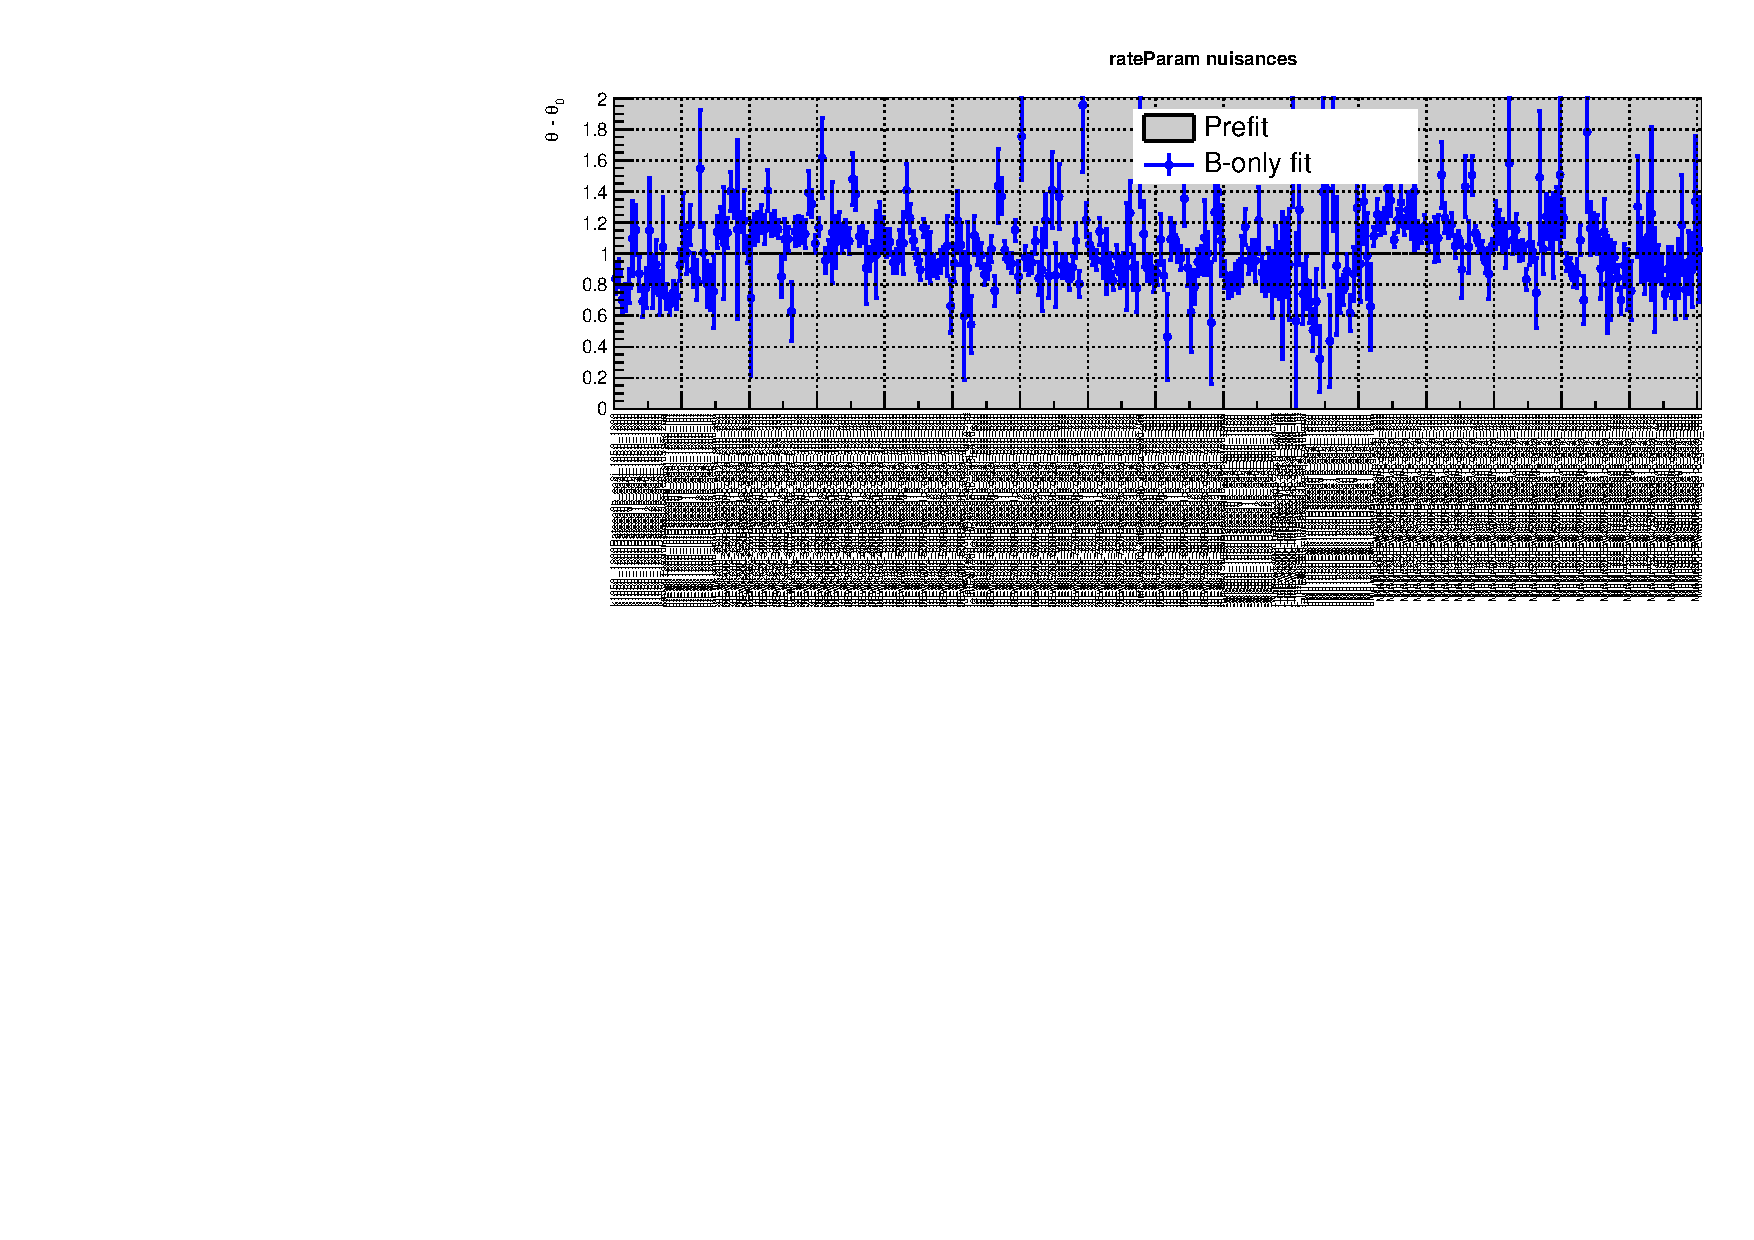
\includegraphics[width=1.\linewidth]{figures/results/36invfb/prefit/nuis/Rates_nuisances}
%\end{figure}
%
%\begin{figure}[h!]
%  \centering
%  \caption{Correlated sources of uncertainty}
%  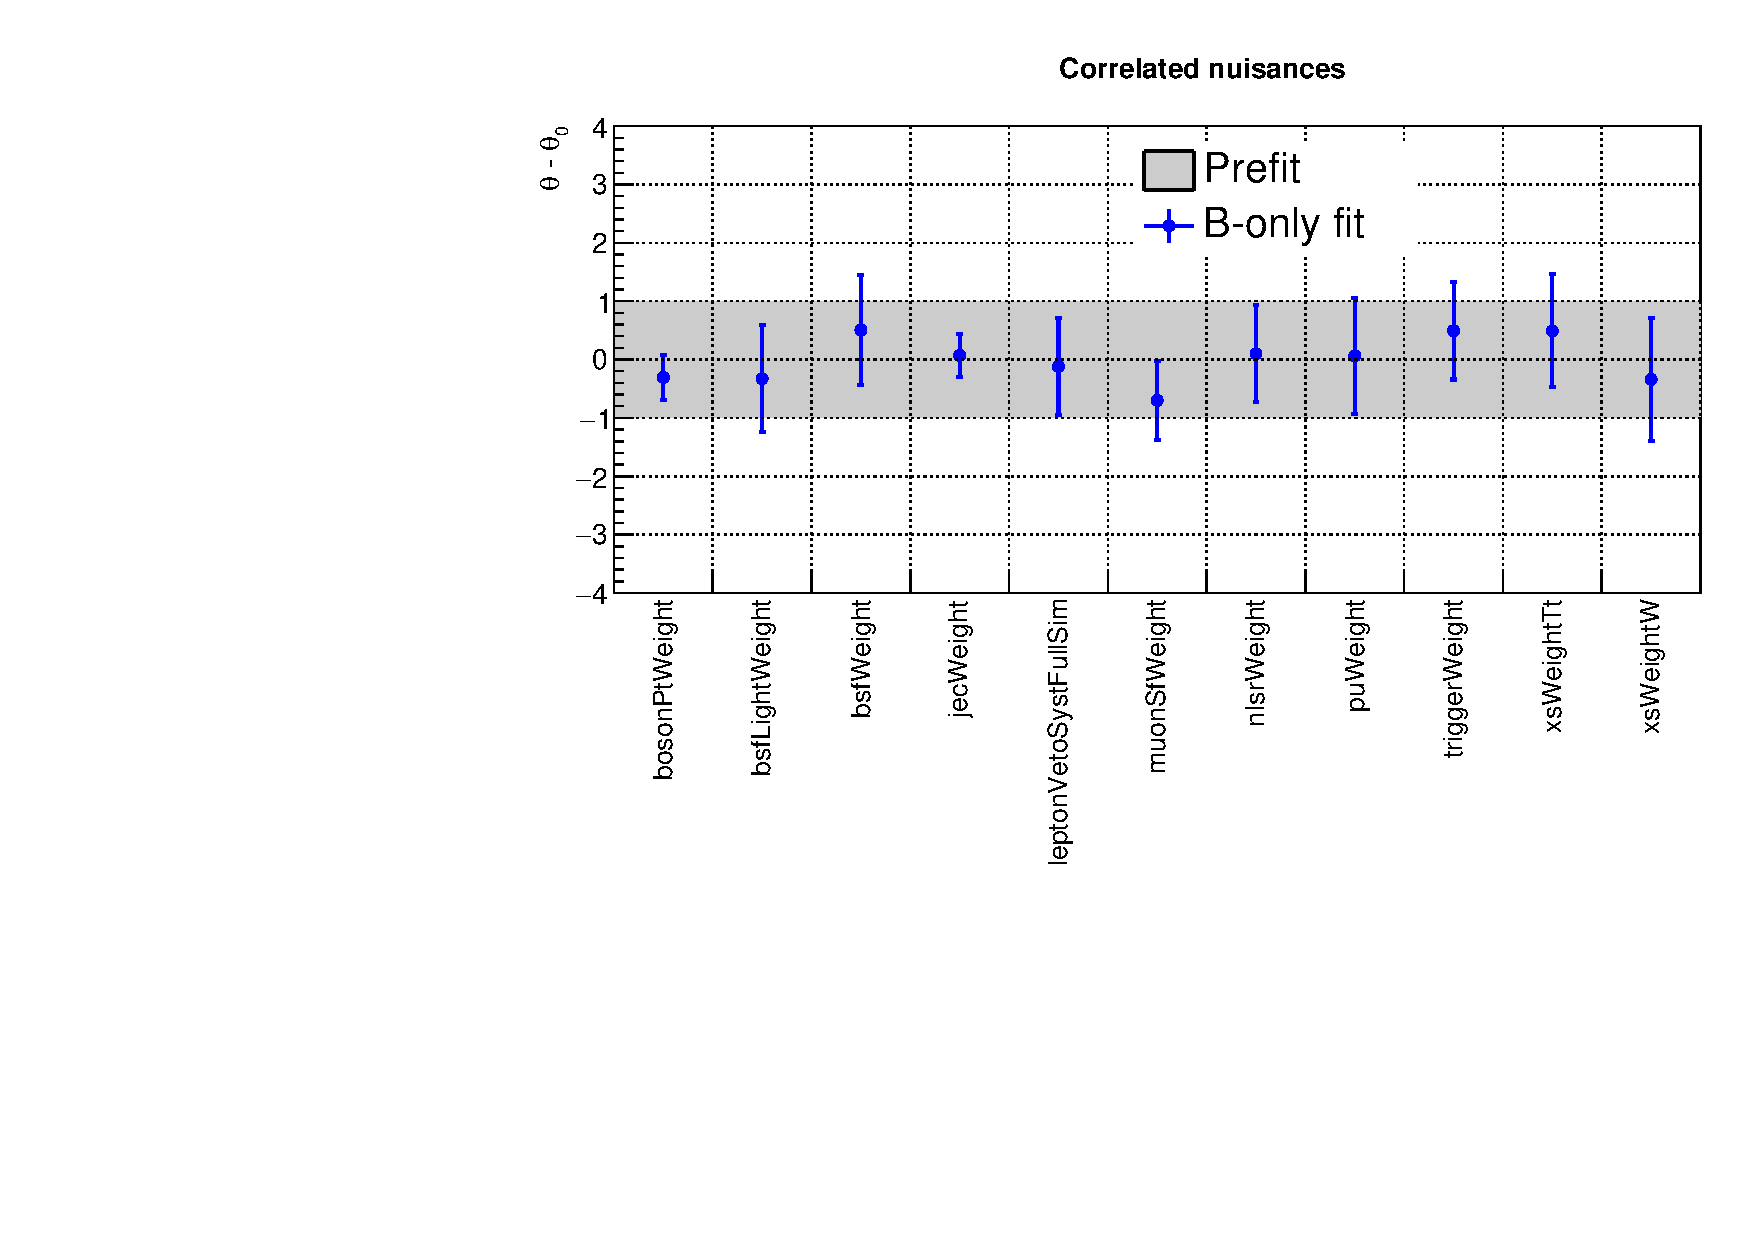
\includegraphics[width=1.\linewidth]{figures/results/36invfb/prefit/nuis/Correlated_nuisances}
%\end{figure}

\clearpage
\subsection{Post-fit nuisance parameters}
\label{app:nuispost}

\begin{figure}[h!]
  \centering
  \caption{Rate parameters}
  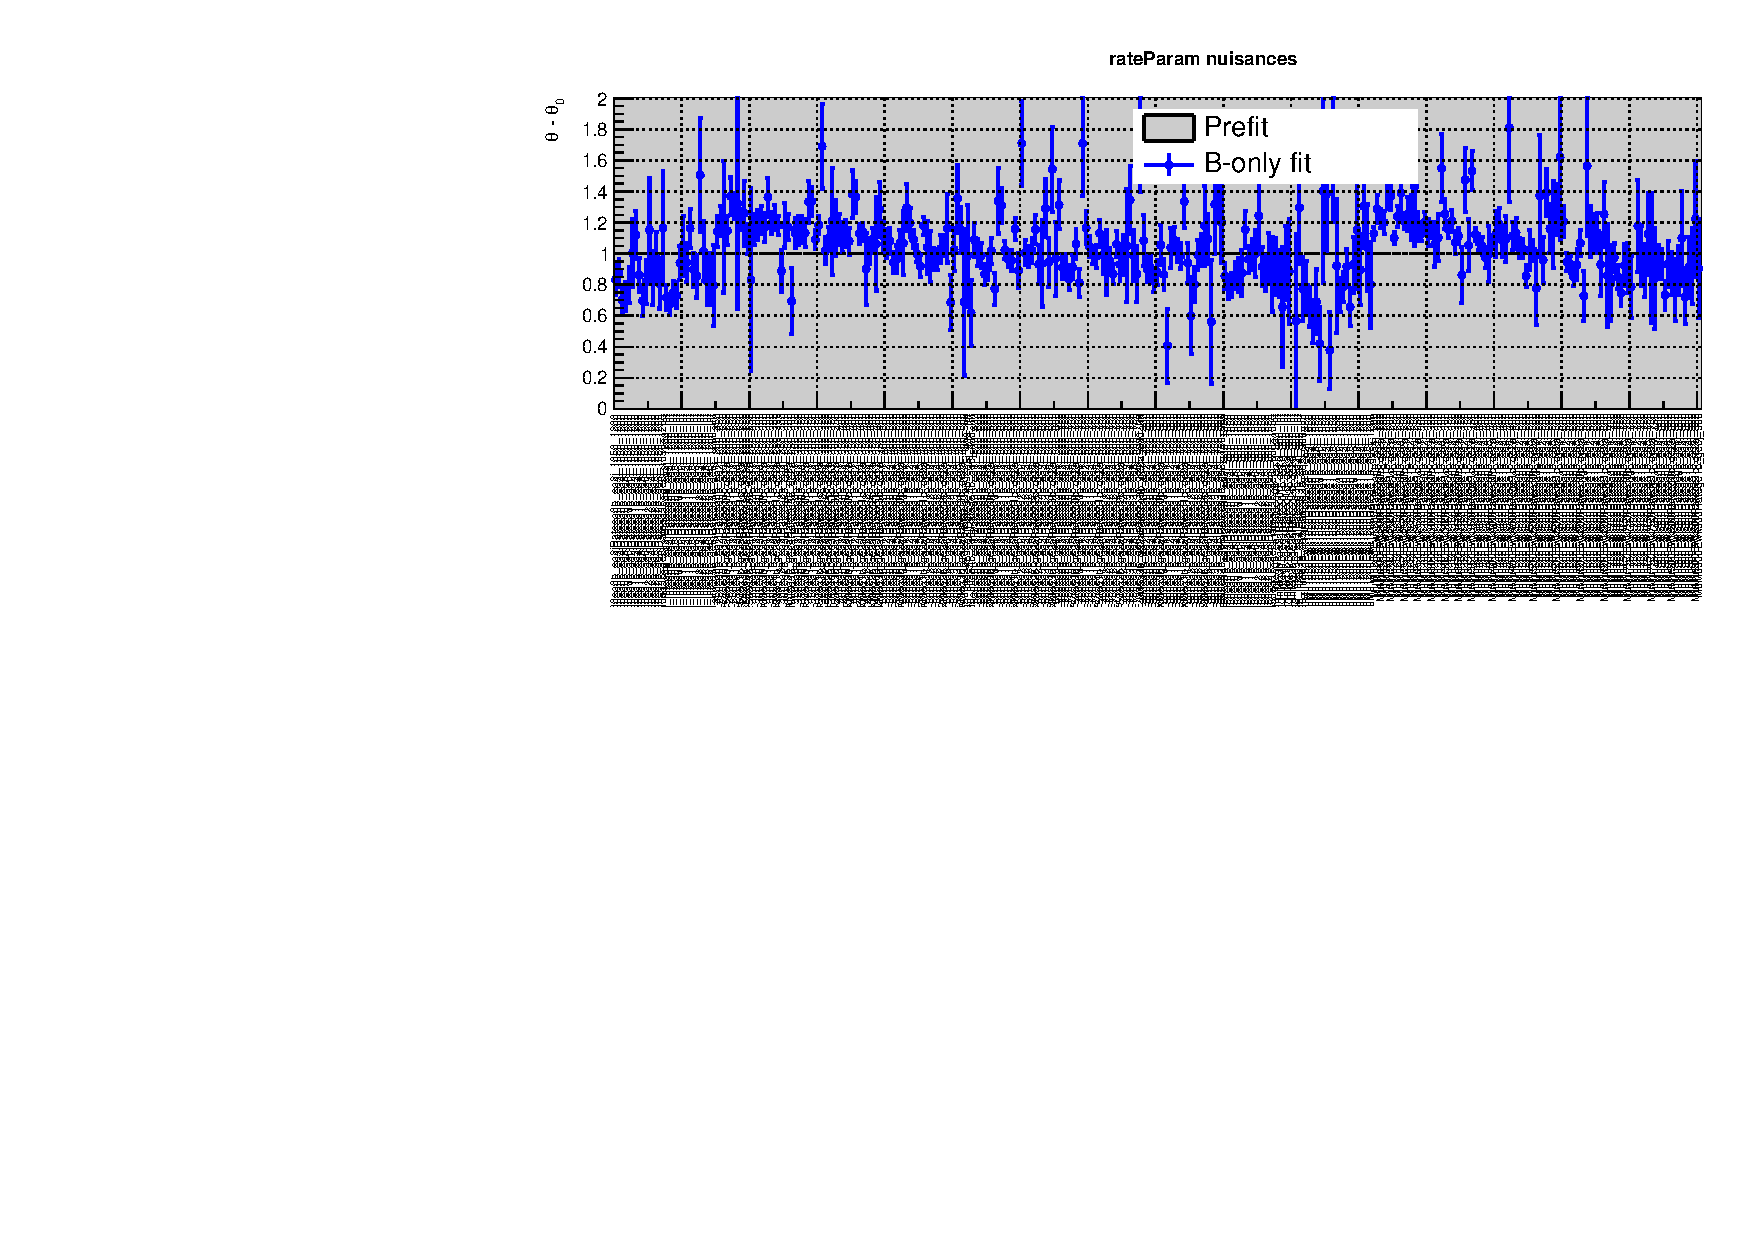
\includegraphics[width=1.\linewidth]{figures/results/36invfb_preapproval/postfit/nuis/Rates_nuisances}
\end{figure}

\begin{figure}[h!]
  \centering
  \caption{Correlated sources of uncertainty}
  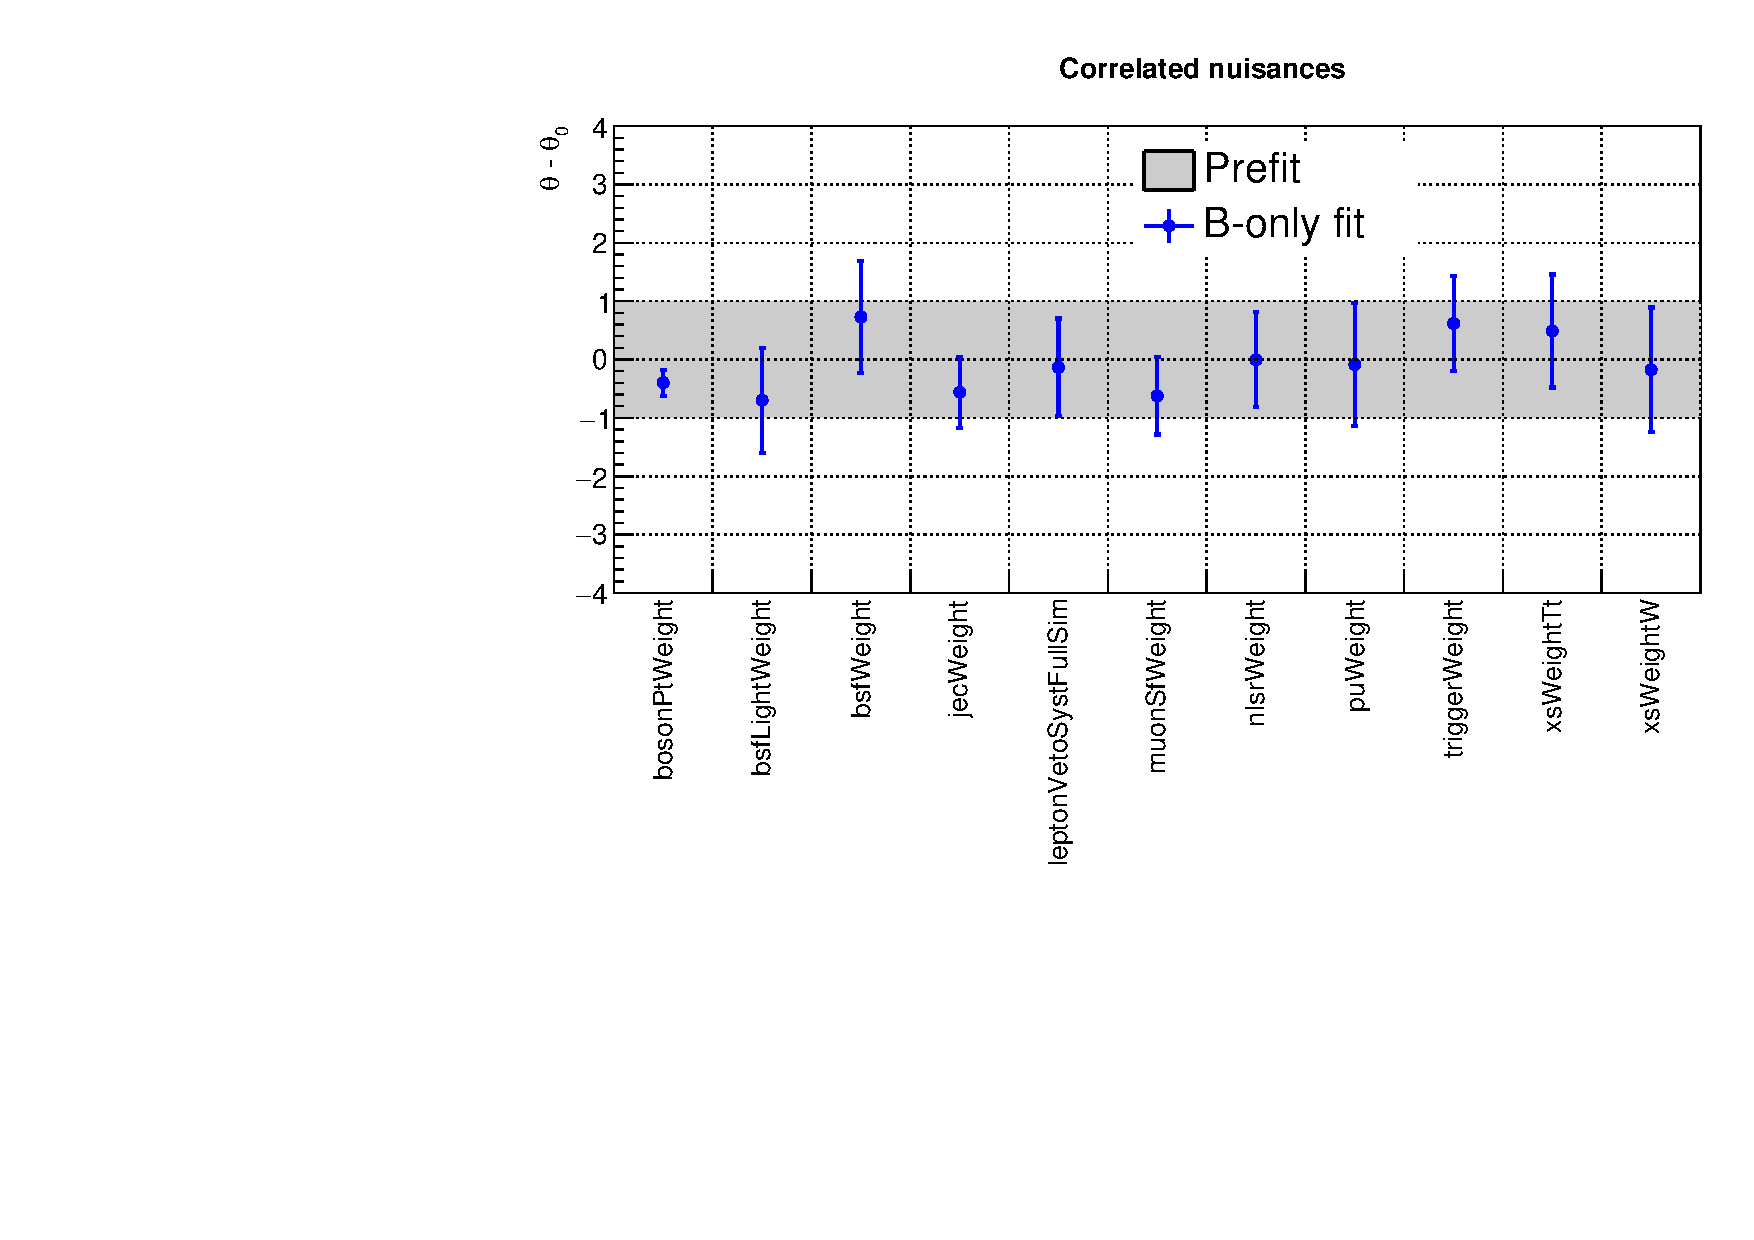
\includegraphics[width=1.\linewidth]{figures/results/36invfb_preapproval/postfit/nuis/Correlated_nuisances}
\end{figure}

\clearpage
\begin{figure}[h!]
  \centering
  \caption{``MC stat.'' uncertainties for lost lepton background.}
  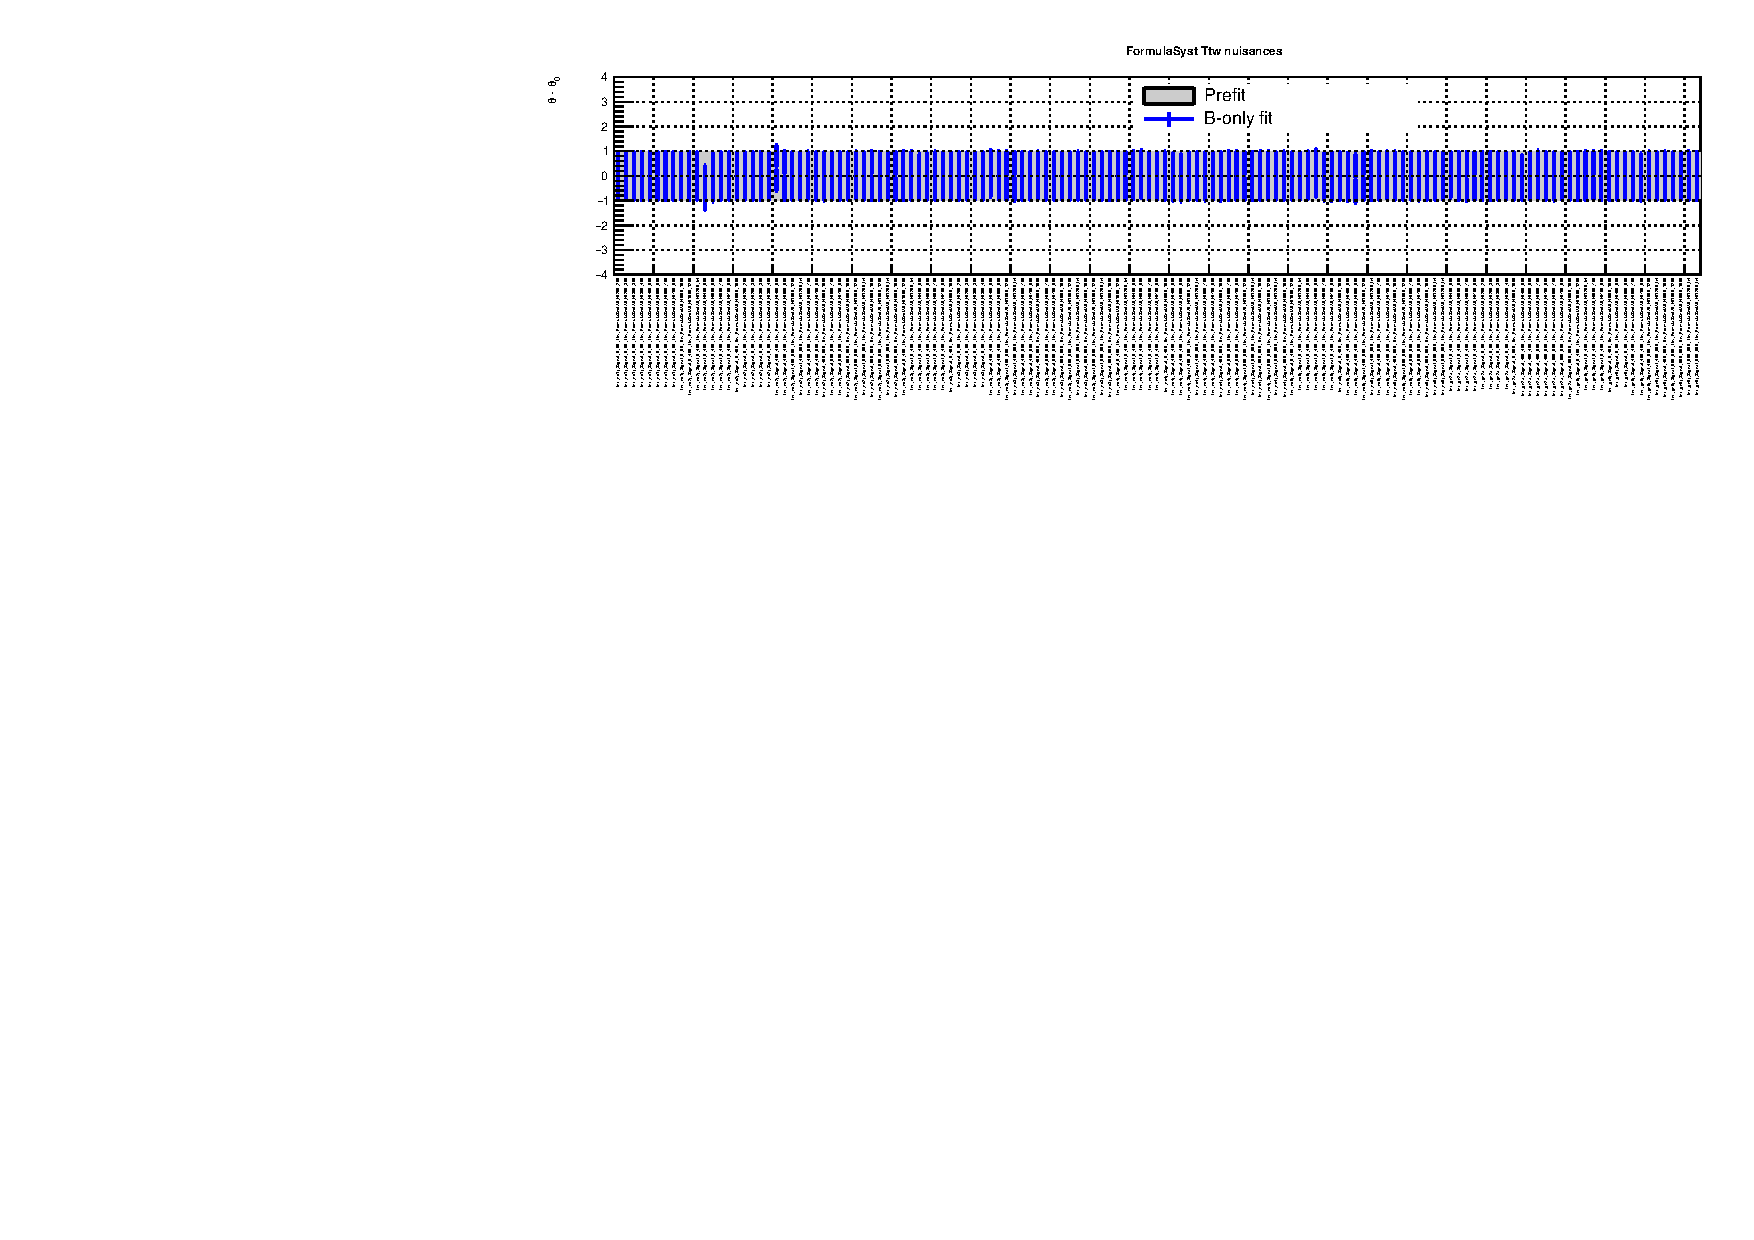
\includegraphics[width=1.\linewidth]{figures/results/36invfb_preapproval/postfit/nuis/FormulaSystTtw_nuisances}
\end{figure}

\begin{figure}[h!]
  \centering
  \caption{``MC stat.'' uncertainties for \znunuj background.}
  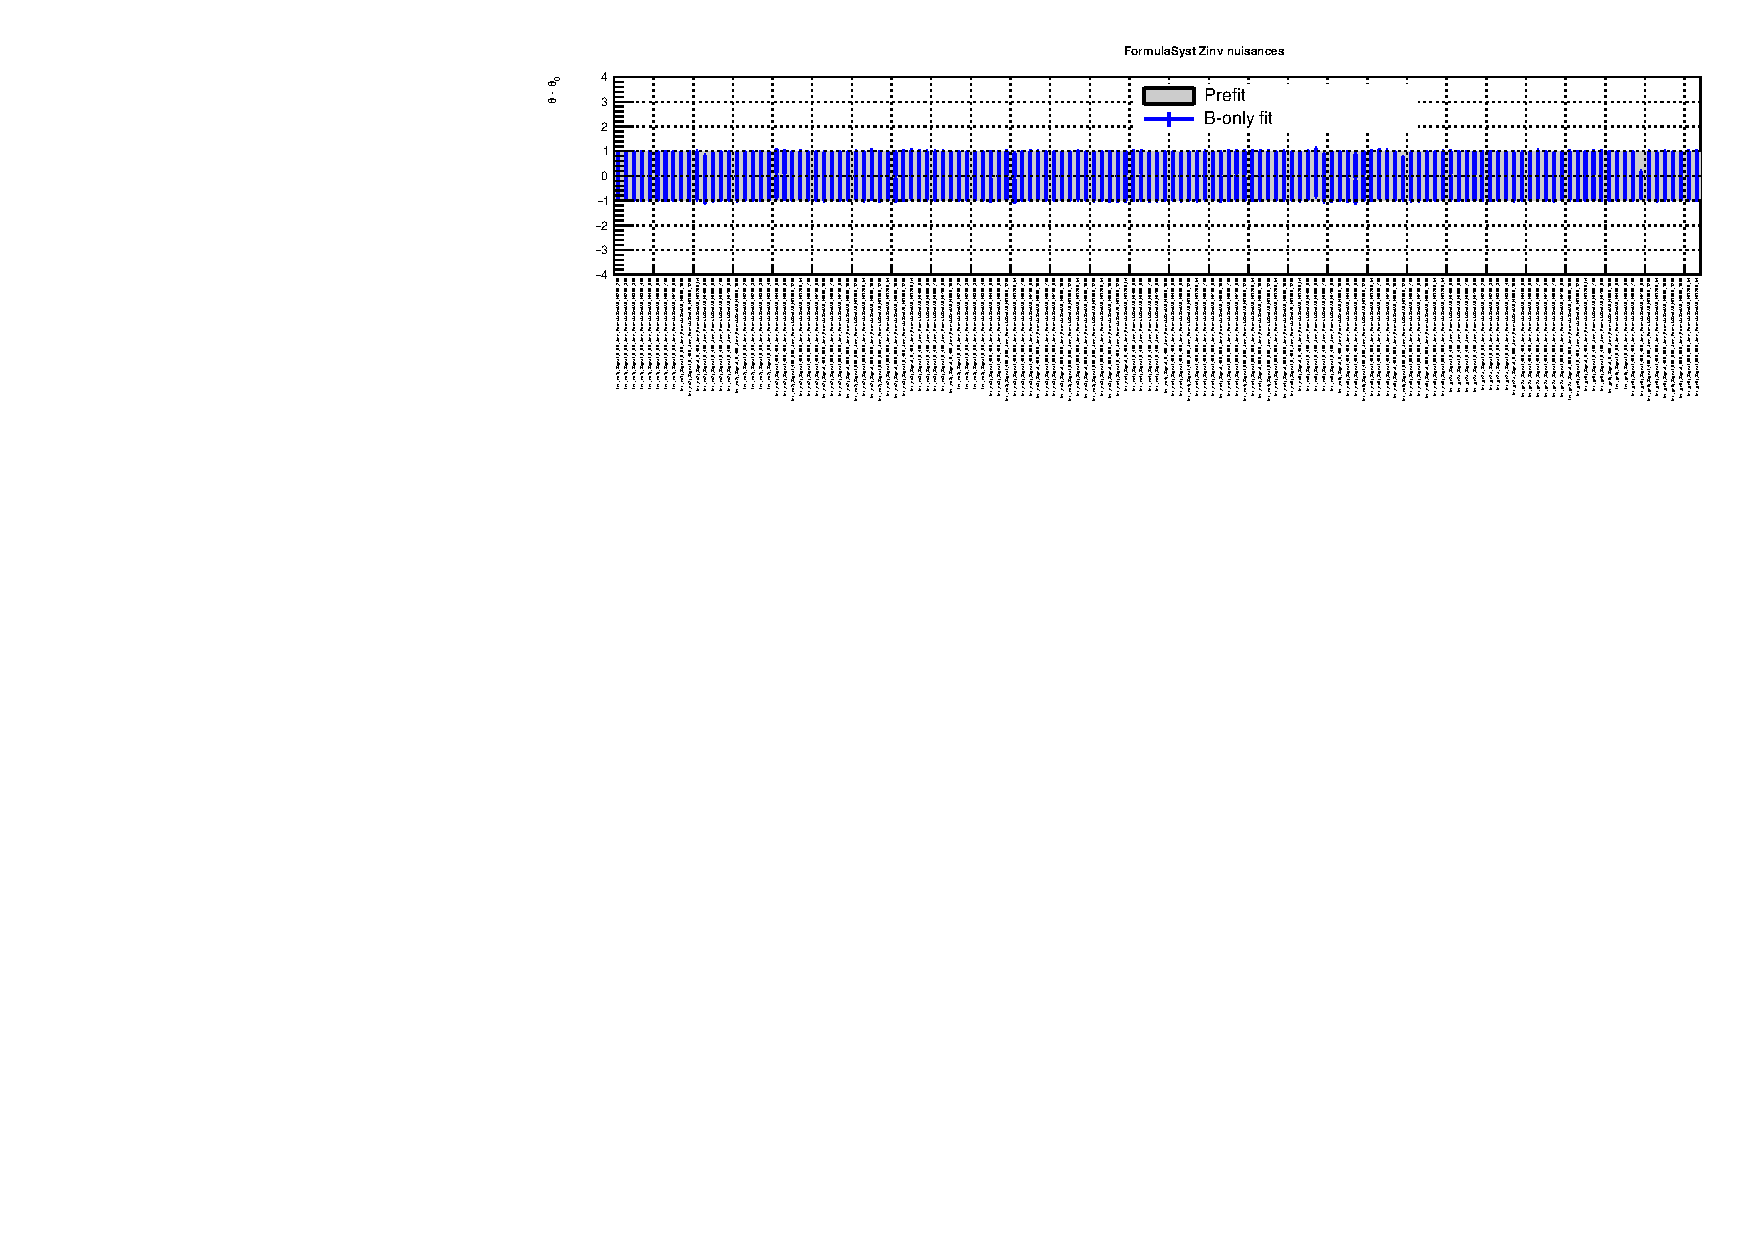
\includegraphics[width=1.\linewidth]{figures/results/36invfb_preapproval/postfit/nuis/FormulaSystZinv_nuisances}
\end{figure}

\clearpage
\begin{figure}[h!]
  \centering
  \caption{Systematic uncertainties in QCD background estimate}
  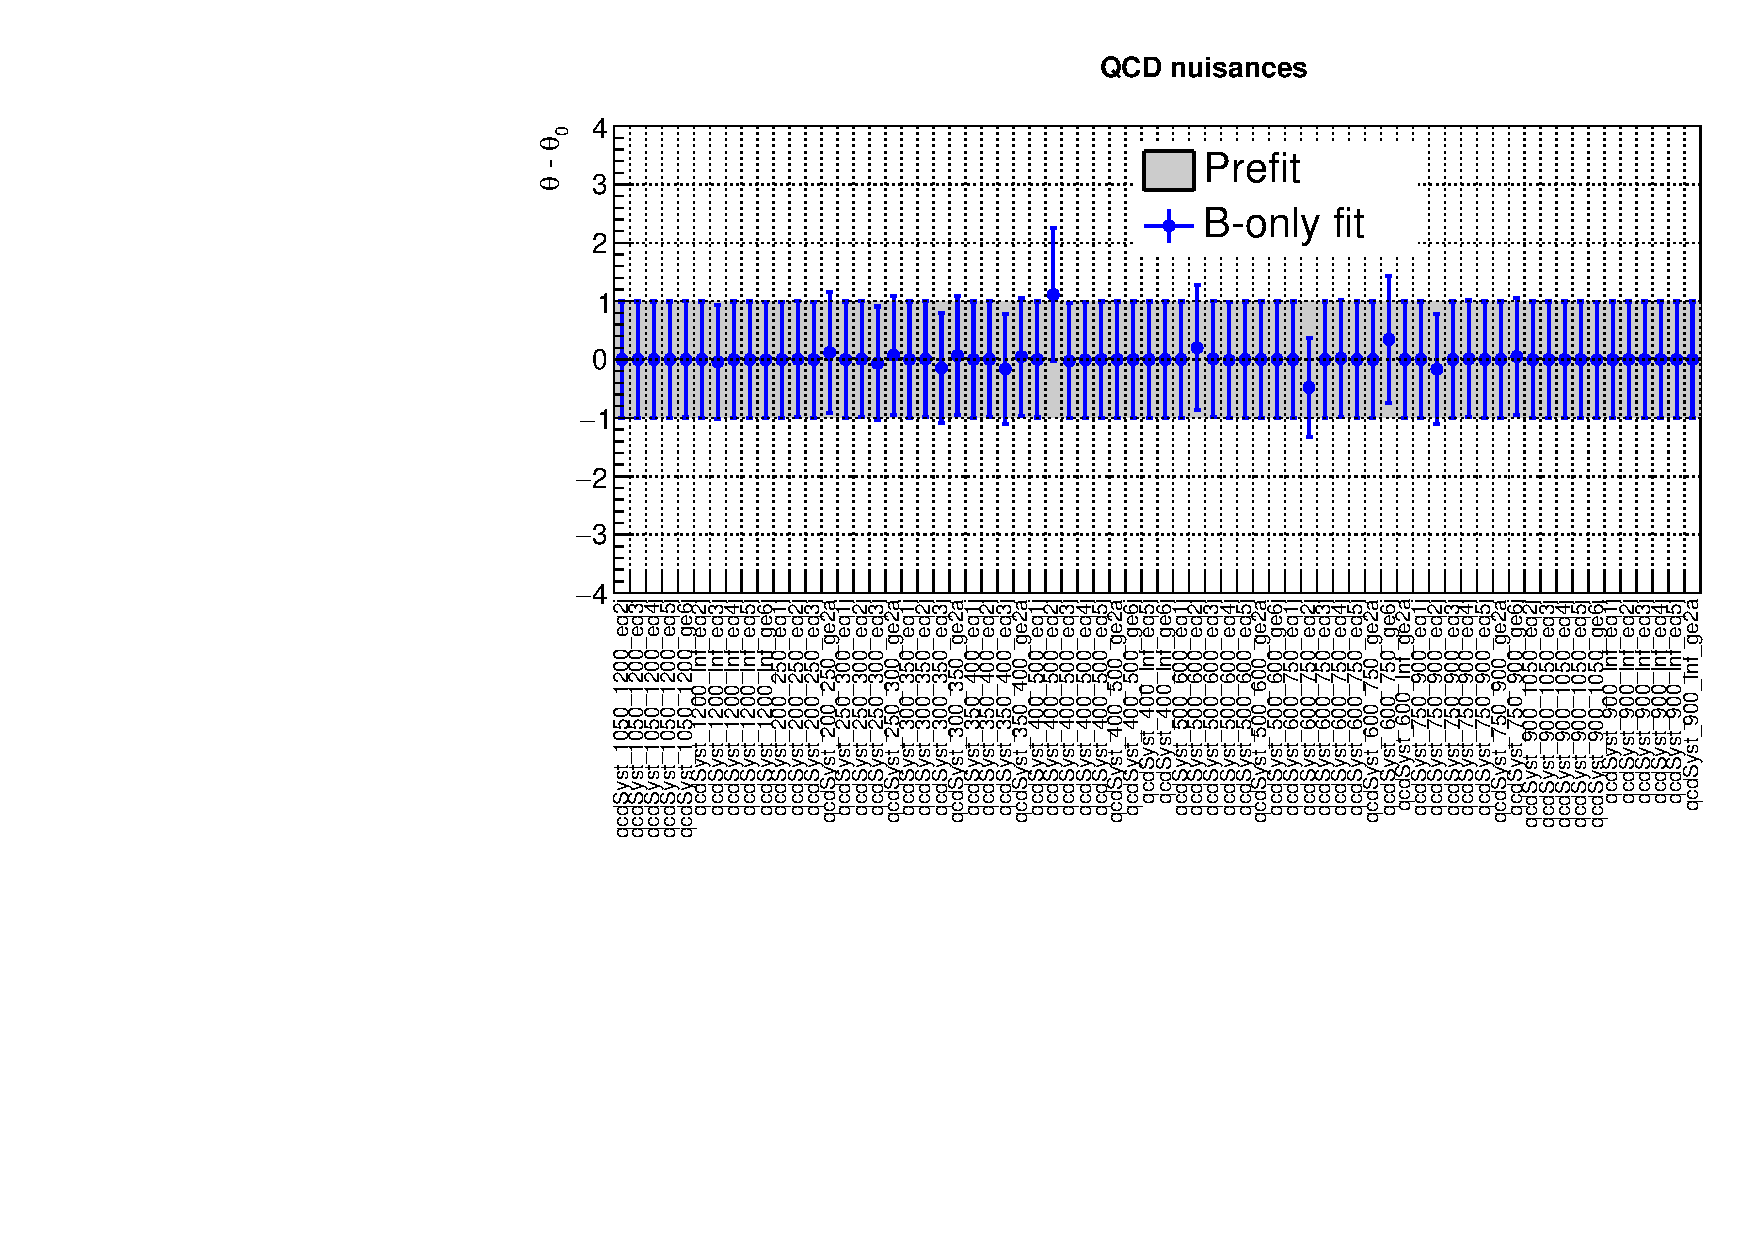
\includegraphics[width=1.\linewidth]{figures/results/36invfb_preapproval/postfit/nuis/qcd_nuisances}
\end{figure}

\clearpage
\begin{figure}[h!]
  \centering
  \caption{Systematic uncertainties per \scalht category in \mht modelling for lost lepton background}
  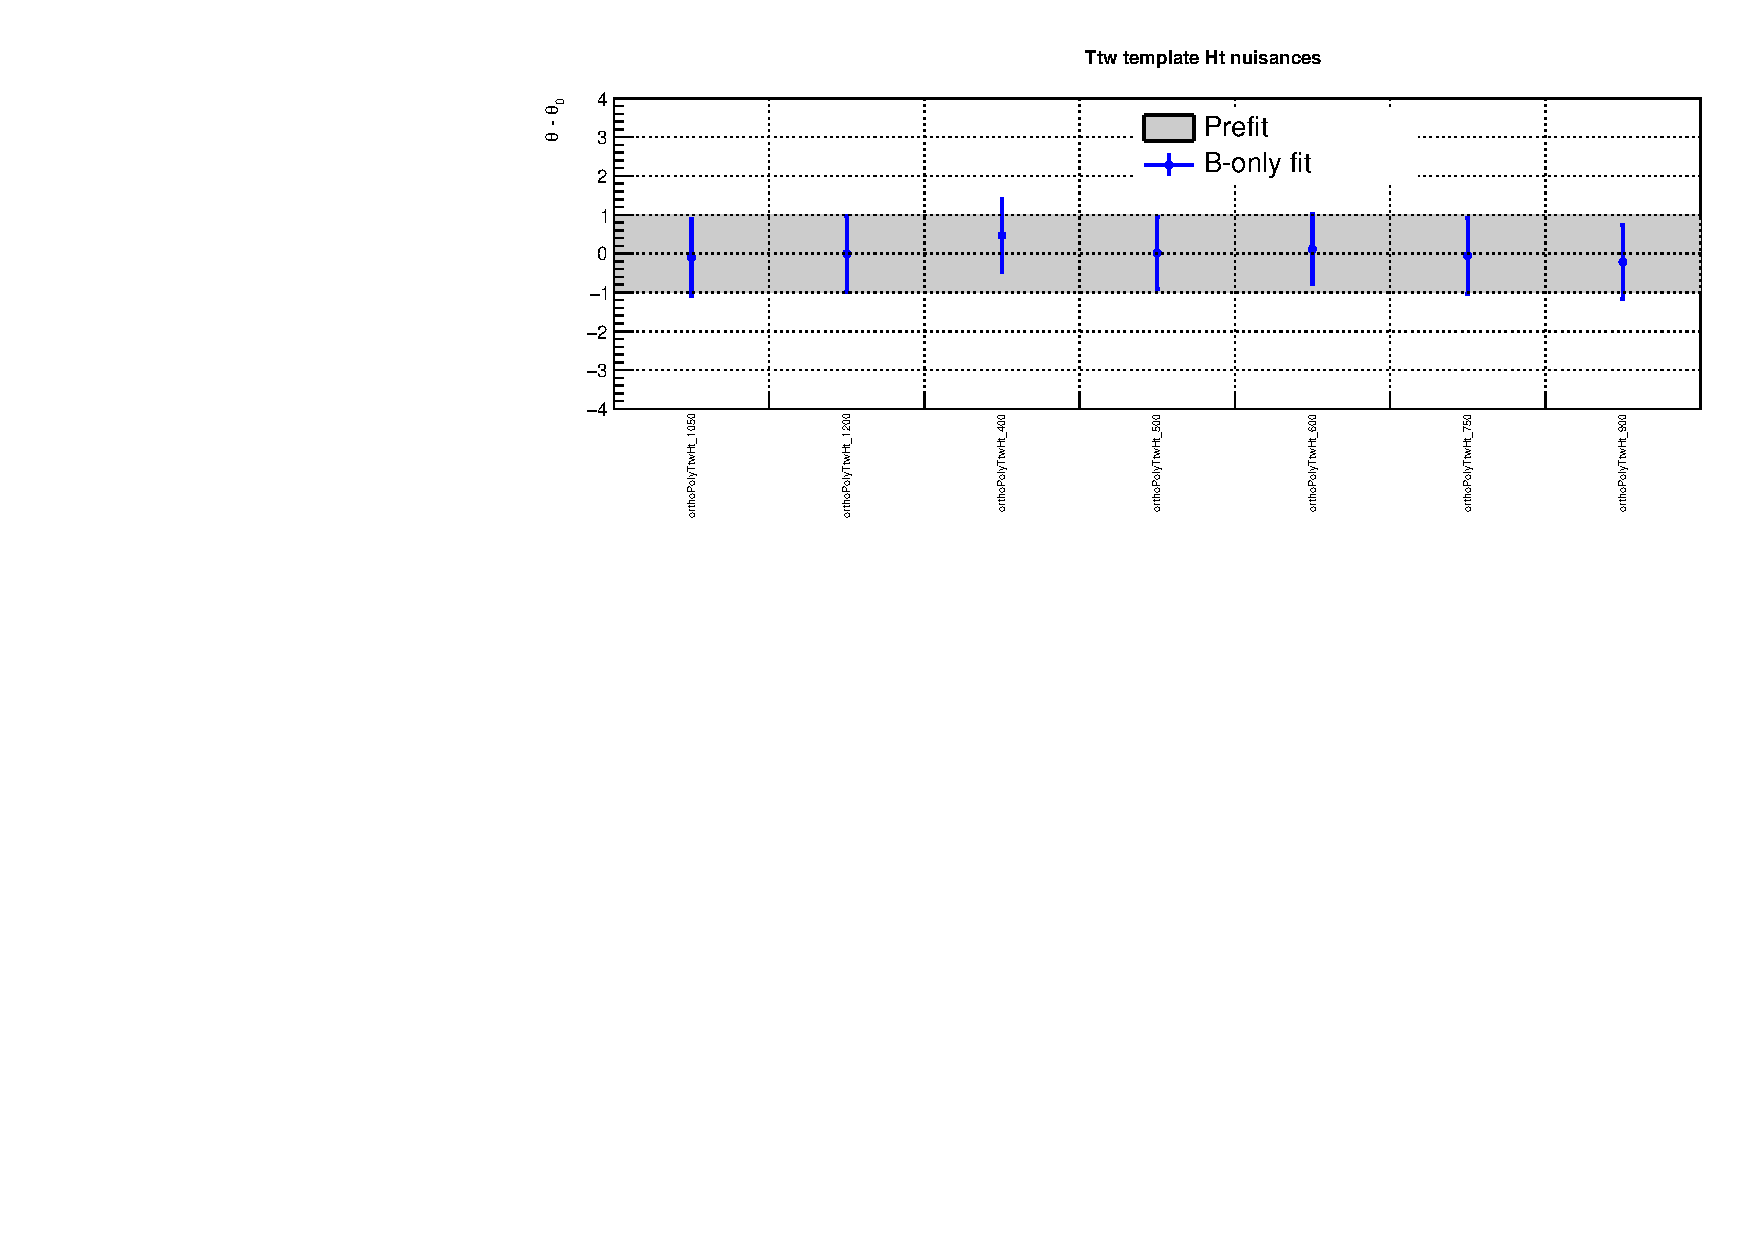
\includegraphics[width=1.\linewidth]{figures/results/36invfb_preapproval/postfit/nuis/TemplateTtw_ht_nuisances}
\end{figure}

\begin{figure}[h!]
  \centering
  \caption{Systematic uncertainties per \njet category in \mht modelling for lost lepton background}
  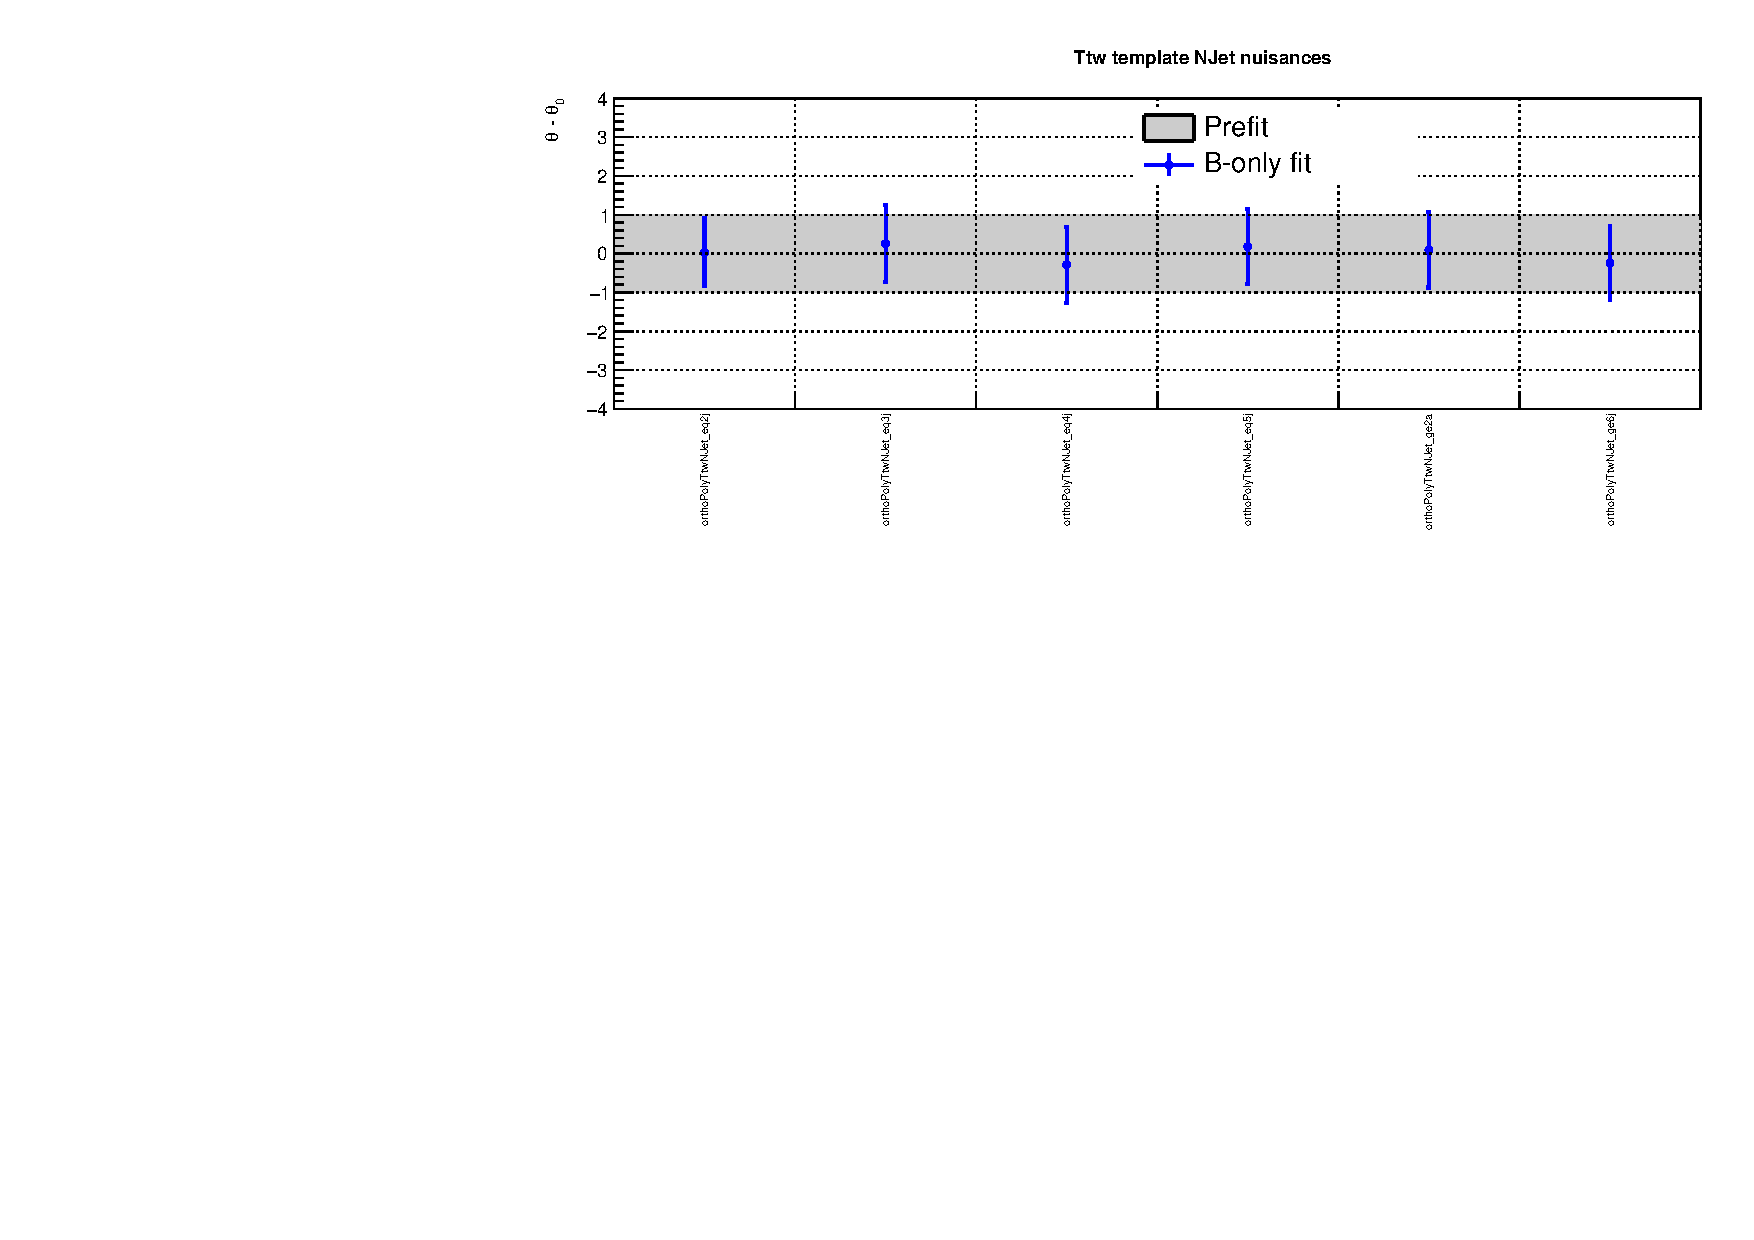
\includegraphics[width=1.\linewidth]{figures/results/36invfb_preapproval/postfit/nuis/TemplateTtw_njet_nuisances}
\end{figure}

\clearpage
\begin{figure}[h!]
  \centering
  \caption{Systematic uncertainties per \scalht category in \mht modelling for \znunuj background}
  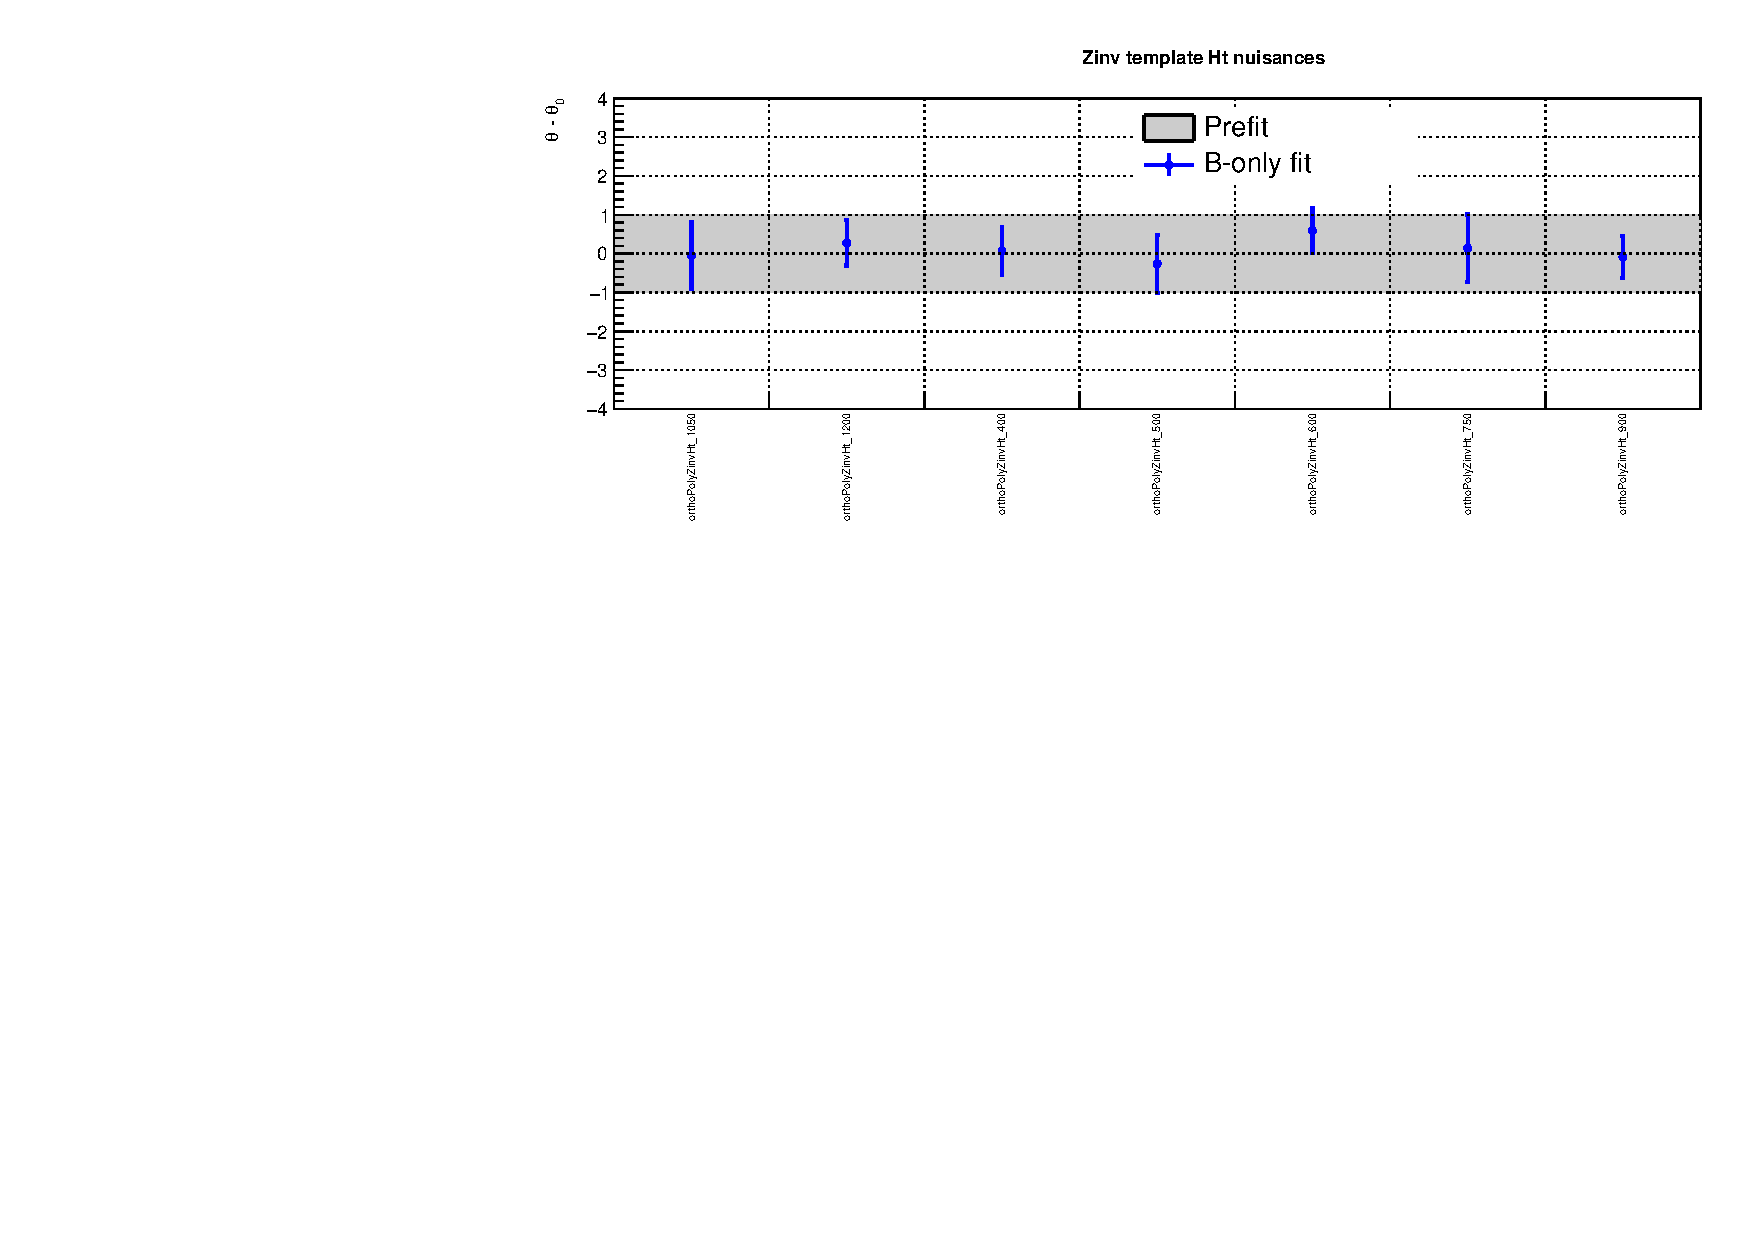
\includegraphics[width=1.\linewidth]{figures/results/36invfb_preapproval/postfit/nuis/TemplateZinv_ht_nuisances}
\end{figure}

\begin{figure}[h!]
  \centering
  \caption{Systematic uncertainties per \njet category in \mht modelling for \znunuj background}
  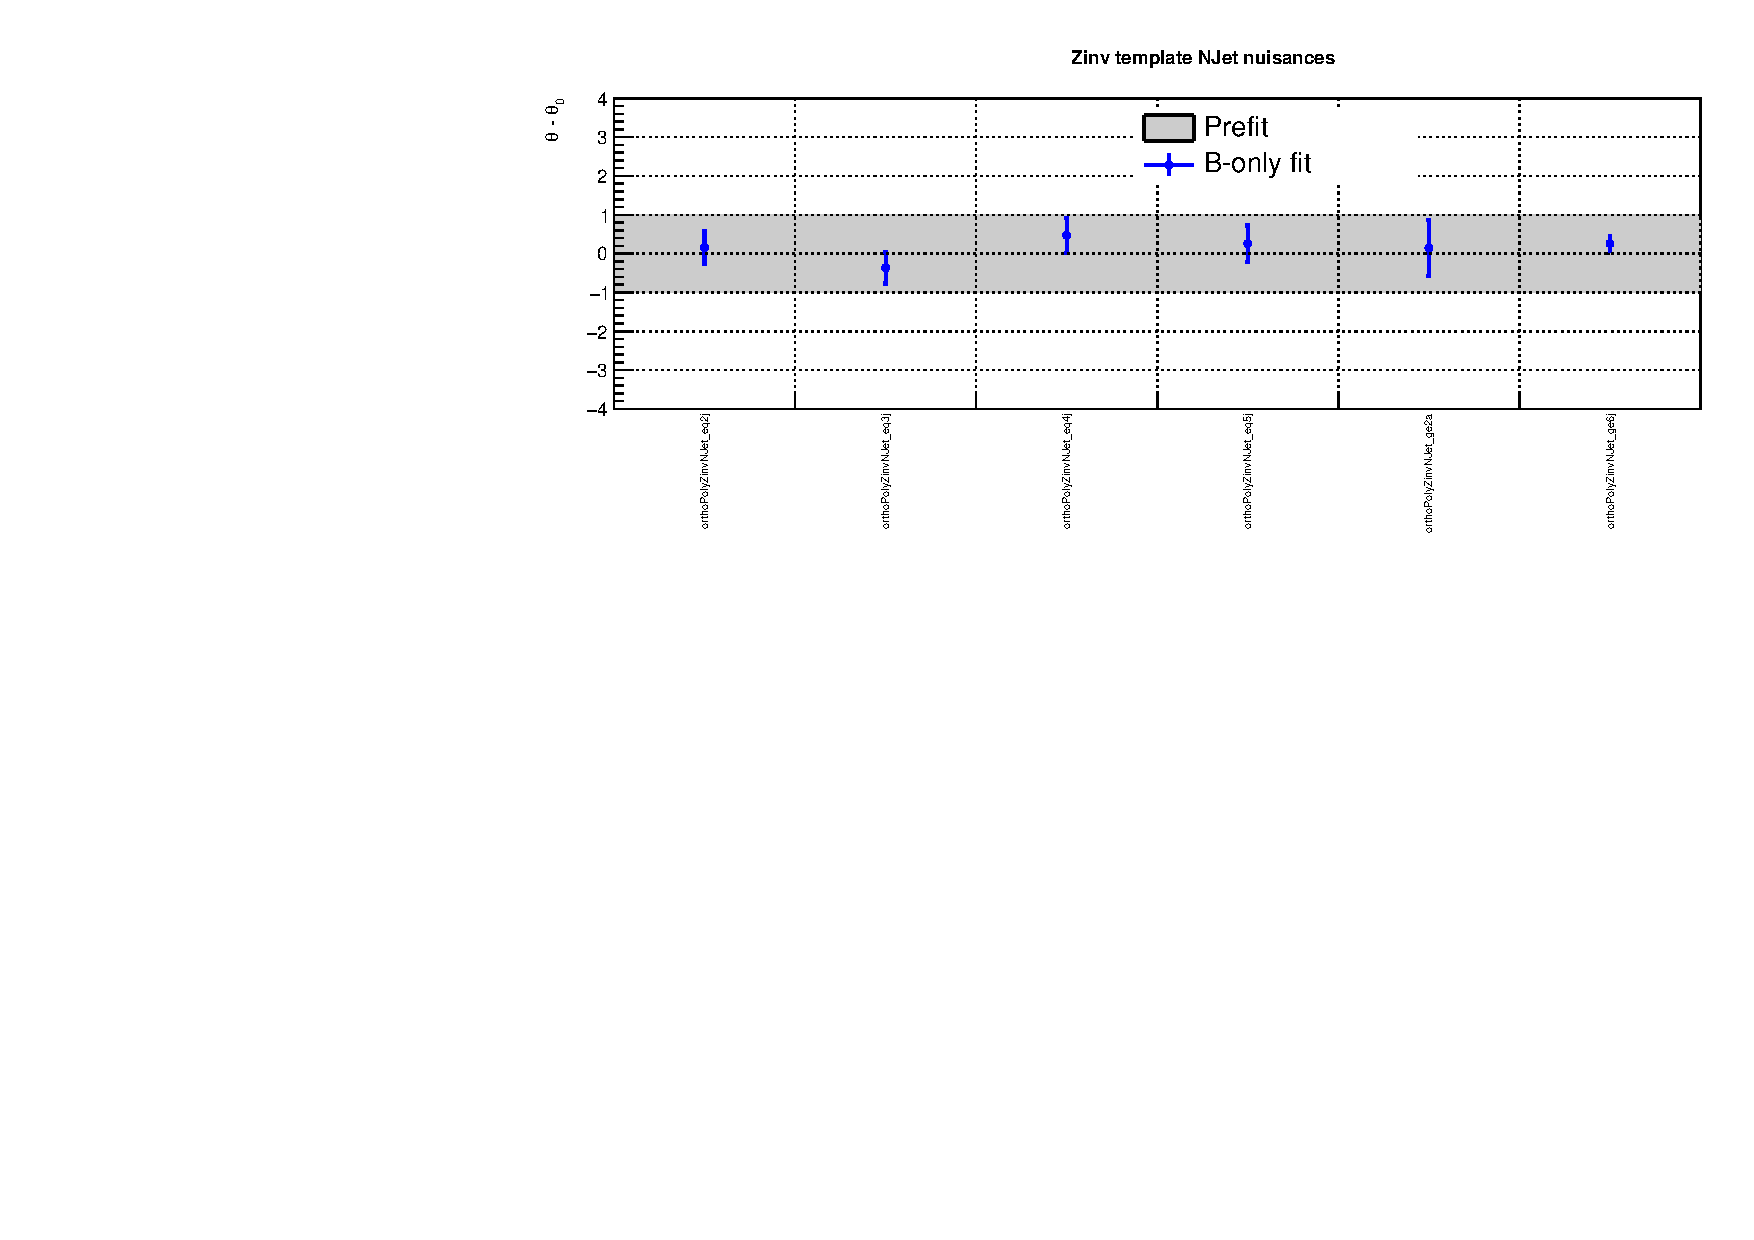
\includegraphics[width=1.\linewidth]{figures/results/36invfb_preapproval/postfit/nuis/TemplateZinv_njet_nuisances}
\end{figure}

\clearpage
\begin{figure}[h!]
  \centering
  \caption{Systematic uncertainties in \alphat modelling}
  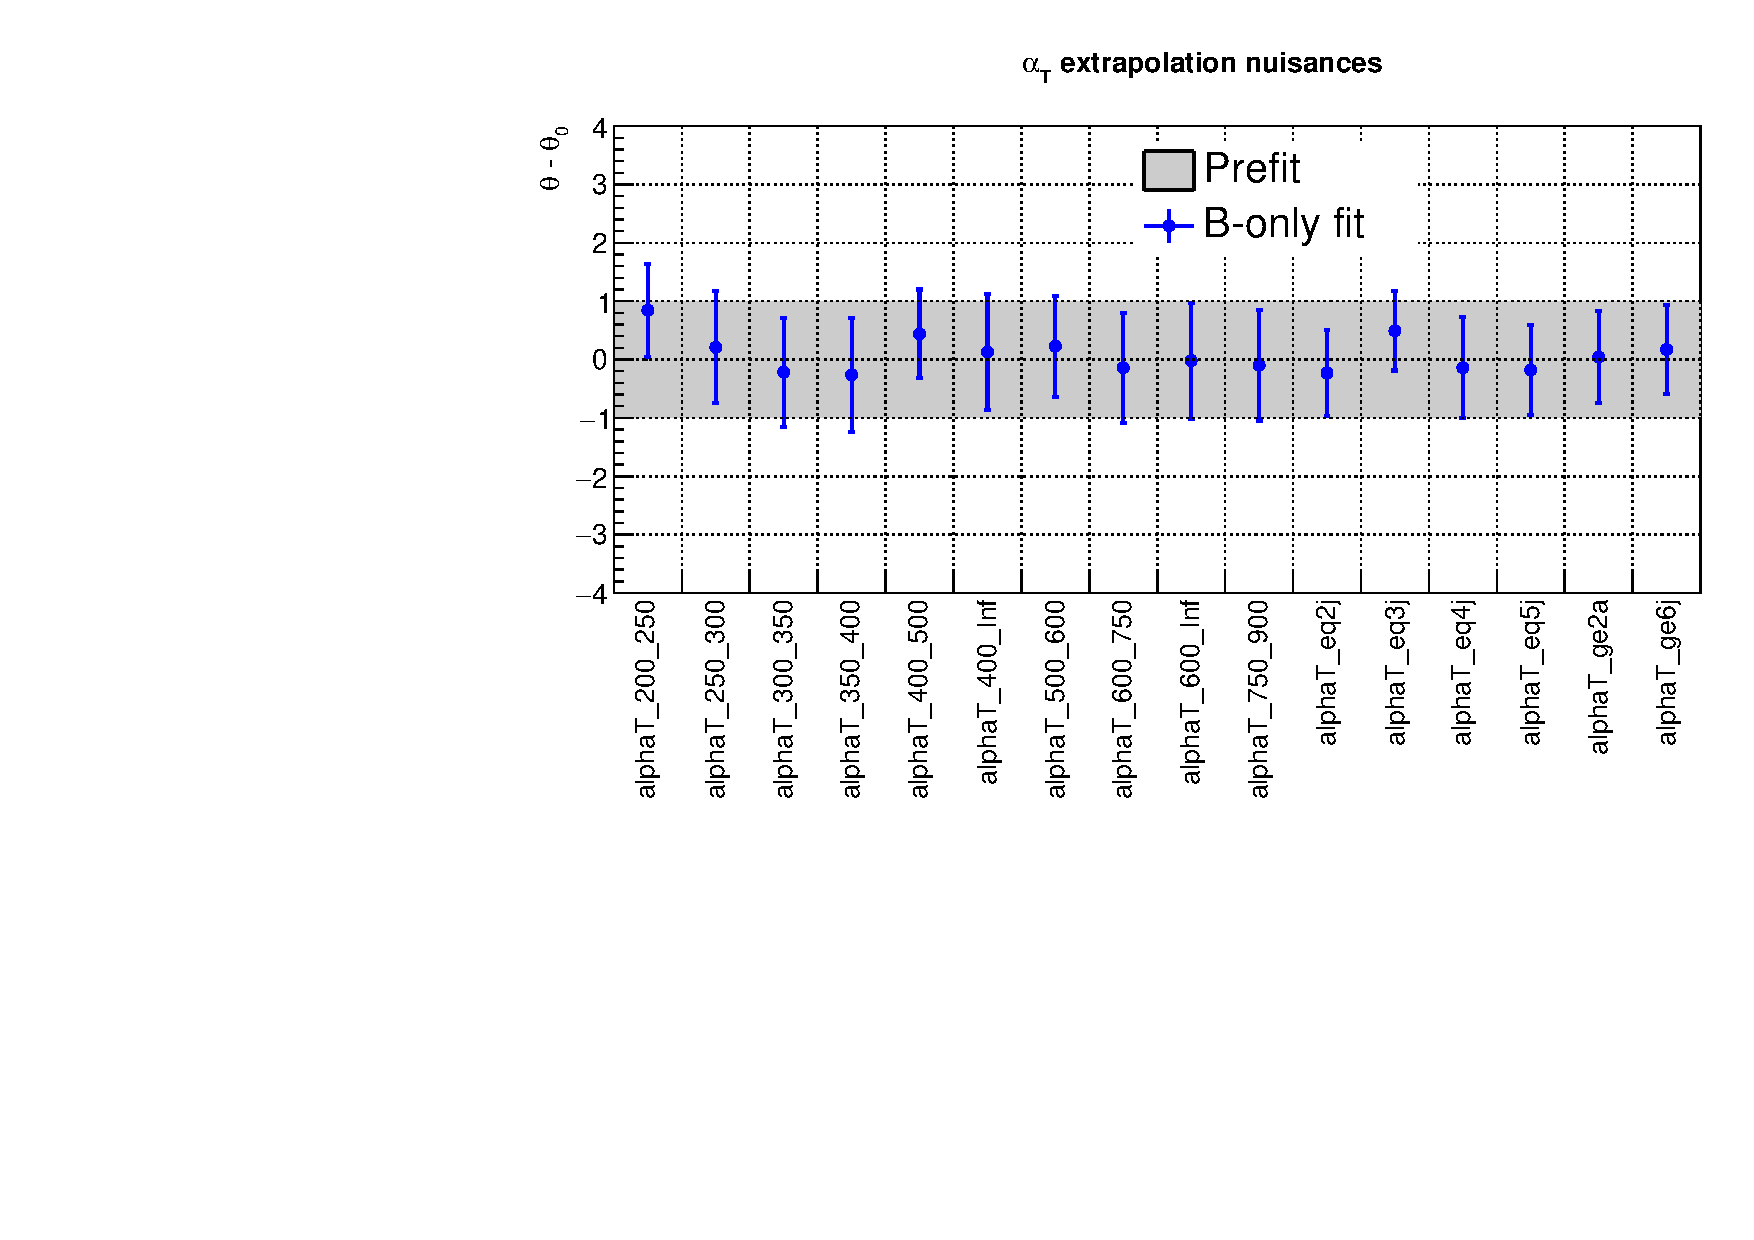
\includegraphics[width=0.8\linewidth]{figures/results/36invfb_preapproval/postfit/nuis/AlphaT_nuisances}
\end{figure}

\begin{figure}[h!]
  \centering
  \caption{Systematic uncertainties in \bdphi modelling}
  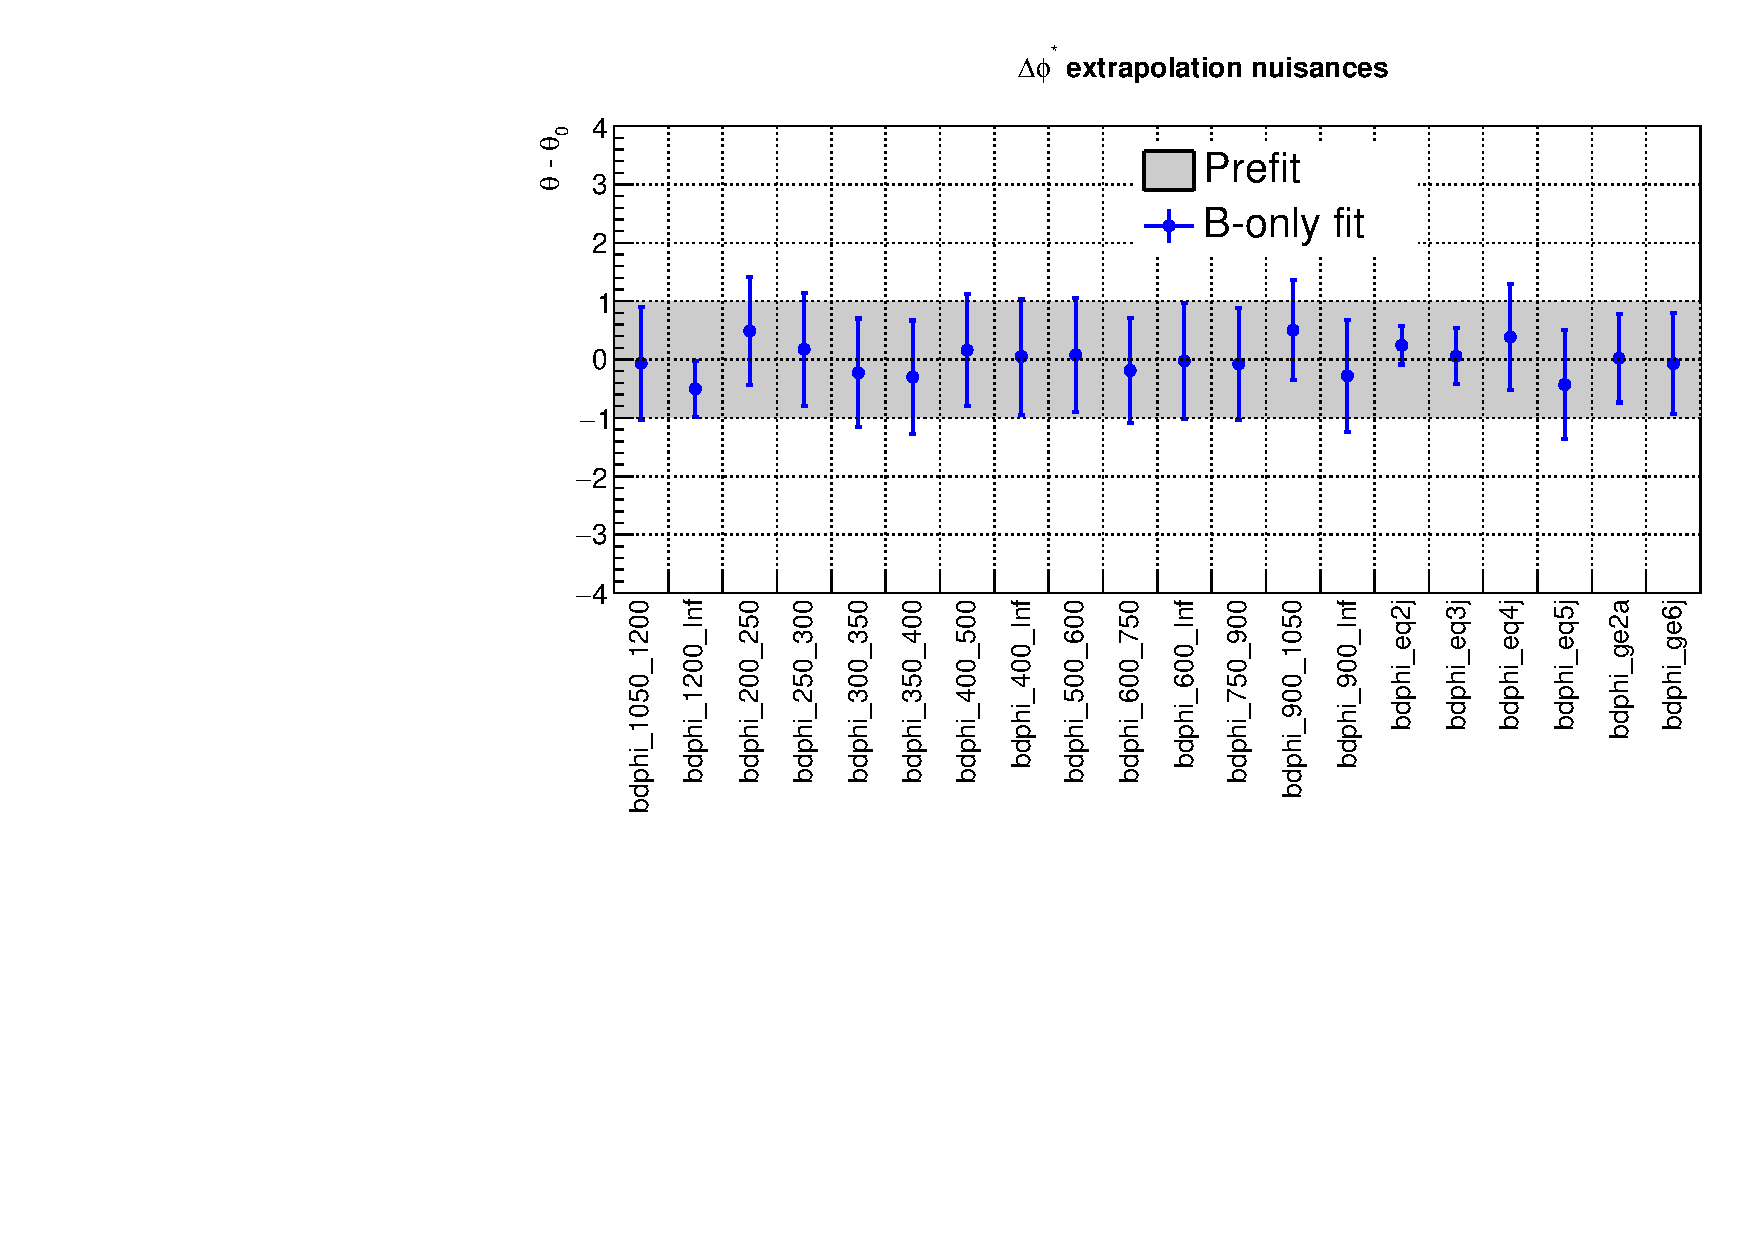
\includegraphics[width=0.8\linewidth]{figures/results/36invfb_preapproval/postfit/nuis/bDPhi_nuisances}
\end{figure}

\clearpage
\begin{figure}[h!]
  \centering
  \caption{Systematic uncertainties in single isolated track veto modelling}
  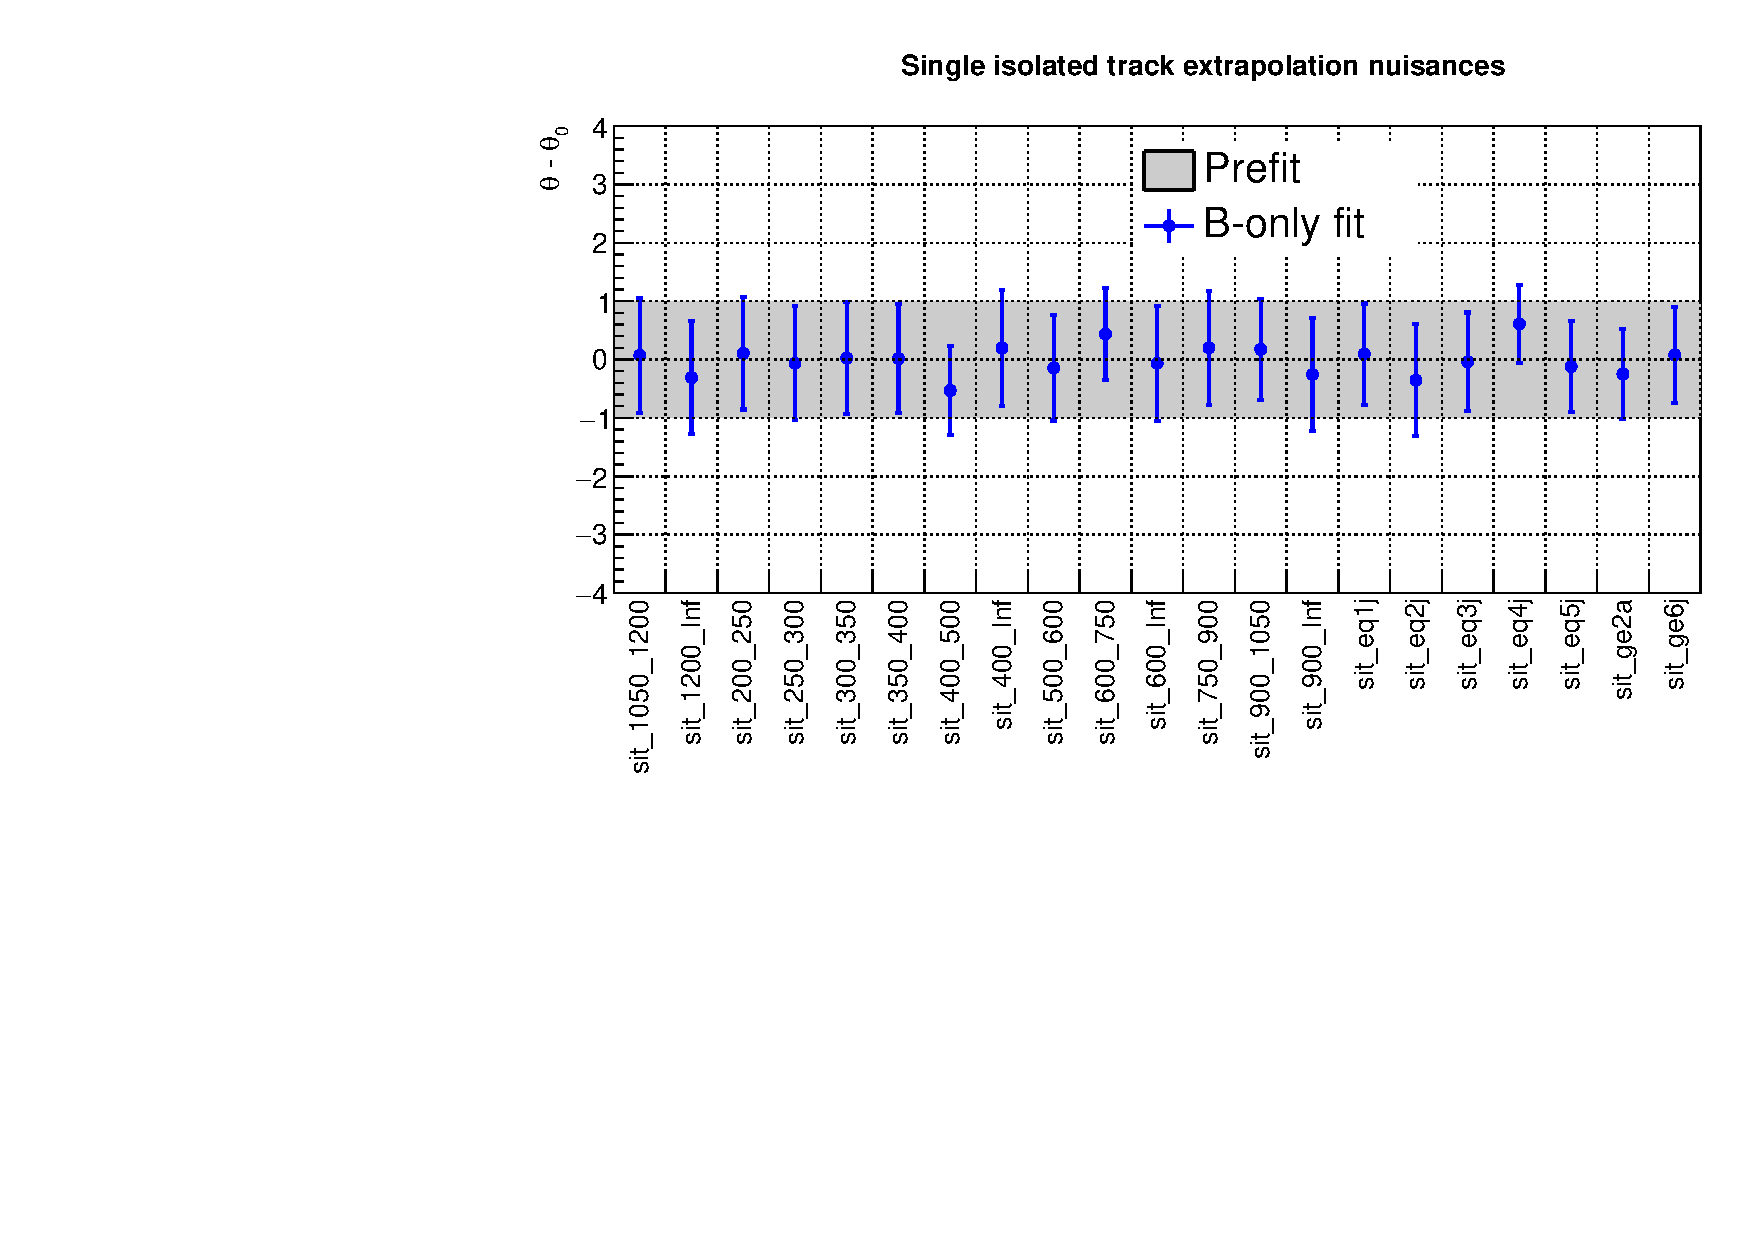
\includegraphics[width=0.8\linewidth]{figures/results/36invfb_preapproval/postfit/nuis/SIT_nuisances}
\end{figure}

\clearpage
\begin{figure}[h!]
  \centering
  \caption{Systematic uncertainties in W polarisation modelling}
  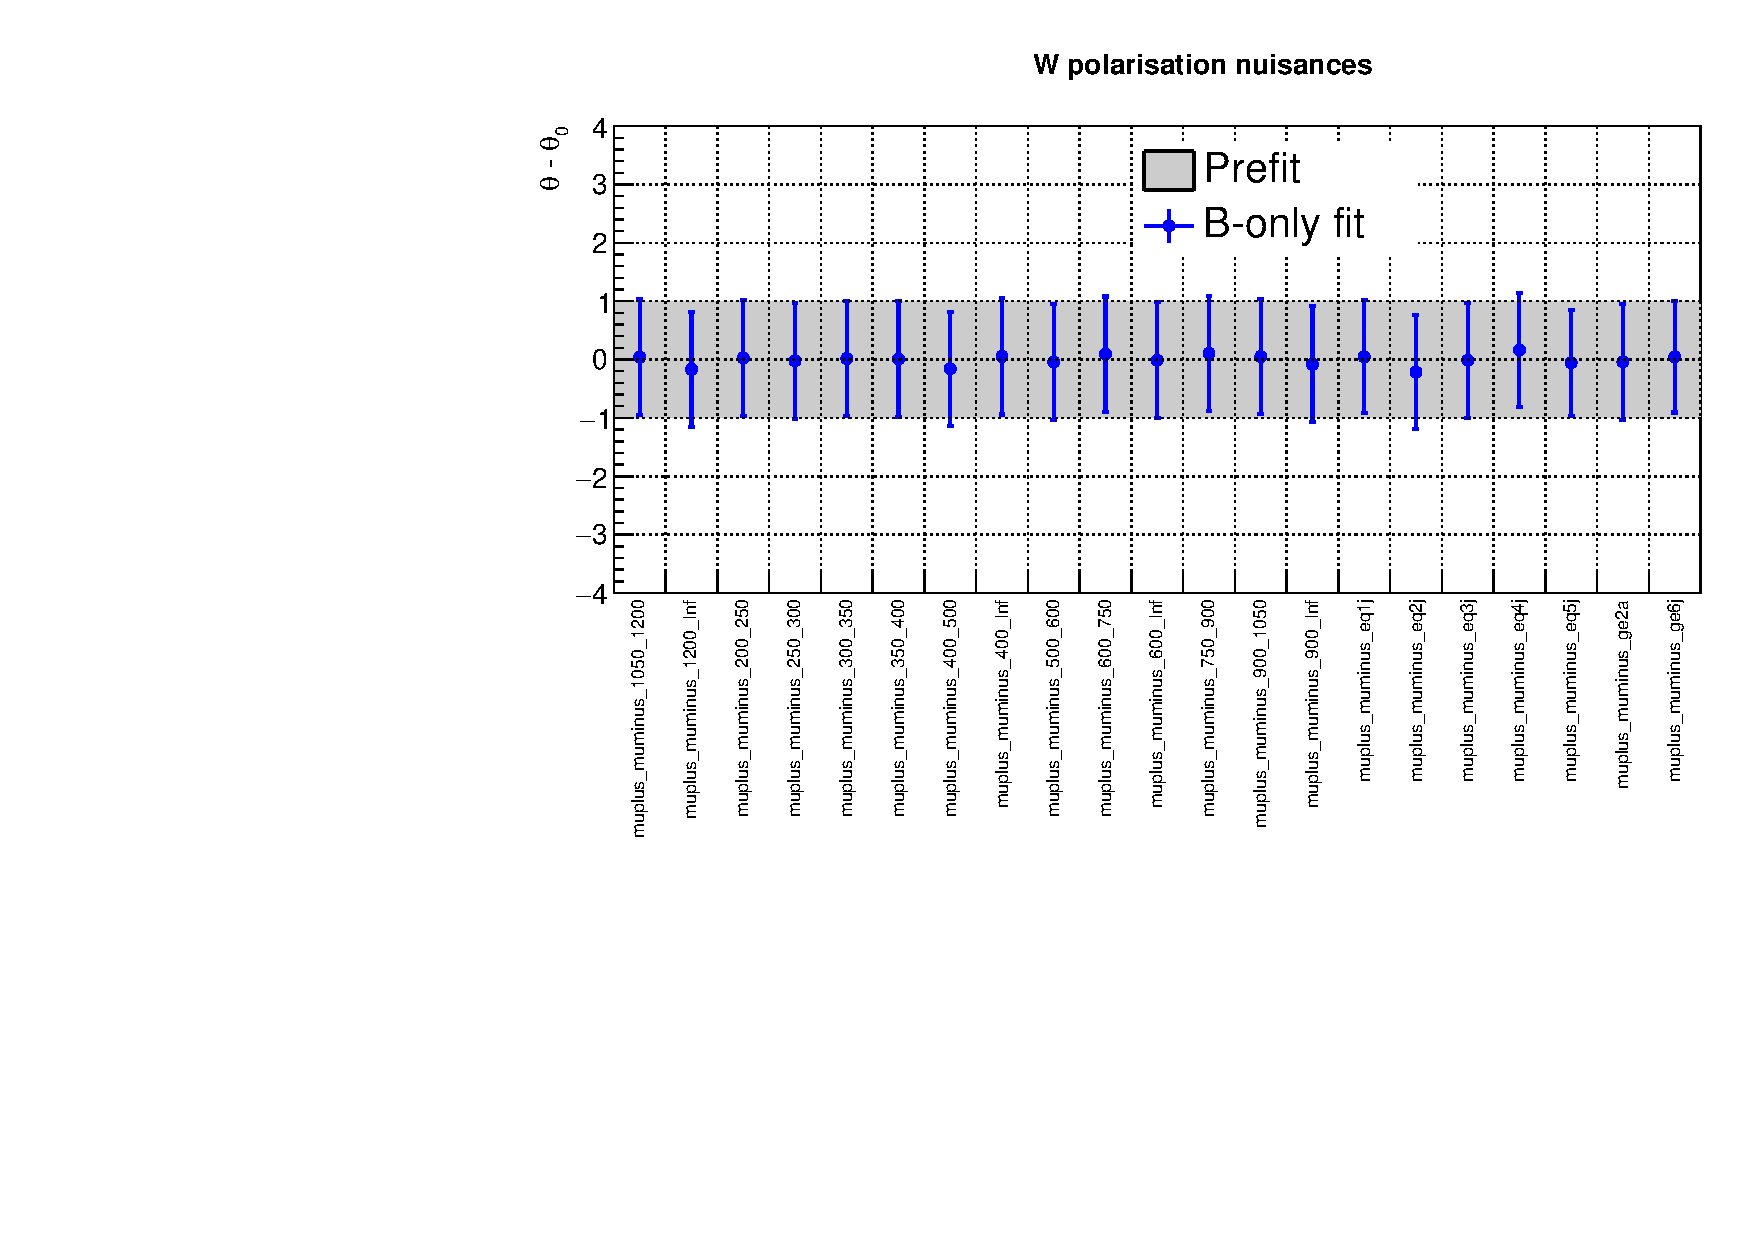
\includegraphics[width=0.8\linewidth]{figures/results/36invfb_preapproval/postfit/nuis/WPol_nuisances}
\end{figure}
